%\documentclass[12pt]{article}
%\documentclass[preprint,prb,aps]{revtex4}
\documentclass[preprint,prb,aps]{revtex4-1}
%\documentclass[preprint,prb,aps]{revtex}
%\sloppy 
\textheight24.0cm                                                              
\textwidth18.0cm                                                               
\topmargin-1.5cm                                                               
\oddsidemargin-1.0cm                                                            
\evensidemargin0.0cm
\usepackage{times}
\usepackage{amsmath}
\usepackage{exscale}
%\usepackage{epsfig}
\usepackage{graphicx}

%\newcommand{\baselinestretch}{2}
\newcommand{\be}[1]{\begin{equation} \label{#1}}
\newcommand{\ee}{\end{equation}}
\newcommand{\bea}[1]{\begin{eqnarray} \label{#1}}
\newcommand{\eea}{\end{eqnarray}}
\newcommand{\bean}{\begin{eqnarray*}}
\newcommand{\eean}{\end{eqnarray*}}

\newcommand{\non}{\nonumber\\}
\newcommand{\eq}[1]{(\ref{#1})}
\newcommand{\difp}[2]{\frac{\partial #1}{\partial #2}}
\newcommand{\br}{{\bf r}}
\newcommand{\bR}{{\bf R}}
\newcommand{\bA}{{\bf A}}
\newcommand{\bB}{{\bf B}}
\newcommand{\bE}{{\bf E}}
%\newcommand{\bm}{{\bf m}}
\renewcommand{\bm}{{\bf m}}
\newcommand{\bn}{{\bf n}}
\newcommand{\bN}{{\bf N}}
\newcommand{\bp}{{\bf p}}
\newcommand{\bP}{{\bf P}}
\newcommand{\bF}{{\bf F}}
\newcommand{\by}{{\bf y}}
\newcommand{\bz}{{\bf z}}
\newcommand{\bZ}{{\bf Z}}
\newcommand{\bV}{{\bf V}}
\newcommand{\bv}{{\bf v}}
\newcommand{\bu}{{\bf u}}
\newcommand{\bx}{{\bf x}}
\newcommand{\bX}{{\bf X}}
\newcommand{\bW}{{\bf W}}
\newcommand{\bJ}{{\bf J}}
\newcommand{\bj}{{\bf j}}
\newcommand{\bk}{{\bf k}}
\newcommand{\bTheta}{{\bf \Theta}}
\newcommand{\btheta}{{\boldsymbol\theta}}
\newcommand{\bOmega}{{\bf \Omega}}
\newcommand{\bomega}{{\boldsymbol\omega}}
\newcommand{\brho}{{\boldsymbol\rho}}
\newcommand{\rd}{{\rm d}}
\newcommand{\rJ}{{\rm J}}
\newcommand{\cA}{{\cal A}}
\newcommand{\cR}{{\cal R}}
\newcommand{\cZ}{{\cal Z}}
\newcommand{\ph}{{\varphi}}
\newcommand{\te}{\theta}
\newcommand{\tht}{\vartheta}
\newcommand{\vpar}{v_\parallel}
\newcommand{\vparkb}{v_{\parallel k b}}
\newcommand{\vparkm}{v_{\parallel k m}}
\newcommand{\Jpar}{J_\parallel}
\newcommand{\ppar}{p_\parallel}
\newcommand{\Bpstar}{B_\parallel^*}
\newcommand{\intpi}{\int\limits_{0}^{2\pi}}
\newcommand{\summ}{\sum \limits_{m=-\infty}^\infty}
\newcommand{\tb}{\tau_b(\uv)}
\newcommand{\bh}{{\bf h}}
\newcommand{\cE}{{\cal E}}
\newcommand{\bsigma}{{\boldsymbol\sigma}}
\newcommand{\bS}{{\mathbf S}}
\newcommand{\bI}{{\mathbf I}}
\newcommand{\odtwo}[2]{\frac{\rd #1}{\rd #2}}
\newcommand{\pdone}[1]{\frac{\partial}{\partial #1}}
\newcommand{\pdtwo}[2]{\frac{\partial #1}{\partial #2}}
\newcommand{\ds}{\displaystyle}
%\newcommand{\bc}{\begin{center} 
%\newcommand{\ec}{\end{center}}
%\input{prespan}

\begin{document}

\section{Equilibrium distribution for wide bananas}
\label{sec:maxw}

\noindent
Let's check that in case of constant temperature the following distribution,
\be{equilmaxw}
f_0(H,\psi^\ast)=\frac{\bar n_\alpha(\psi^\ast)}{\left(2\pi m_\alpha T_\alpha\right)^{3/2}}
\exp\left(-\frac{H-e_\alpha\Phi(\psi^\ast)}{T_\alpha}\right),
\ee
where
\be{psiast}
\psi^\ast=\frac{c}{e_\alpha}p_\varphi=\frac{m_\alpha c}{e_\alpha}v_\varphi+A_\varphi
=\frac{m_\alpha c}{e_\alpha}v_\varphi+\psi,
\ee
is a solution to the collisional kinetic equation in all regimes.
Here we use an exact expression for $p_\varphi$ where $v_\varphi$ is the toroidal covariant
component of particle velocity including the Larmor gyration. We also use the exact Hamiltonian
which is
\be{exham}
H=\frac{m_\alpha v^2}{2}+e_\alpha\Phi(\psi)=
\frac{m_\alpha}{2}\left(v_{\rm pol}^2+v_{\rm tor}^2\right)+e_\alpha\Phi(\psi),
\ee
where $v_{\rm tor}=v_\varphi/R$ is a physical toroidal velocity component.
\noindent
Assuming that density and electrostatic potential scale is of the order of plasma radius
we can expand them up to linear order in $m_\alpha c v_\varphi/e_\alpha \ll \psi^a$ where
$\psi^a$ is $\psi$ value at the edge (expansion parameter is then $q R \rho_L / a^2$ where 
$a$ is plasma radius). Thus,
\bea{expand_equilmaxw}
&&\left(2\pi m_\alpha T_\alpha\right)^{3/2} f_0(H,\psi^\ast) 
=
\exp\left(-\frac{1}{T_\alpha}\left(H-e_\alpha\Phi(\psi^\ast)-T_\alpha \log(\bar n_\alpha(\psi^\ast))
\right)\right)
\nonumber \\
&&\approx
\exp\left(-\frac{1}{T_\alpha}\left(H-e_\alpha\Phi(\psi)-T_\alpha \log(\bar n_\alpha(\psi))
-\left(e_\alpha\difp{\Phi(\psi)}{\psi}+\frac{T_\alpha}{\bar n_\alpha}\difp{\bar n_\alpha}{\psi}
\right)\frac{m_\alpha c}{e_\alpha}v_\varphi\right)\right)
\nonumber \\
&&=
\bar n_\alpha(\psi)\exp\left(-\frac{m_\alpha}{T_\alpha}\left(
\frac{1}{2}\left(v_{\rm pol}^2+v_{\rm tor}^2\right)
-\left(\difp{\Phi(\psi)}{\psi}+\frac{T_\alpha}{e_\alpha \bar n_\alpha}\difp{\bar n_\alpha}{\psi}
\right)c R v_{\rm tor}
\right)\right)
\nonumber \\
&&=
\bar n_\alpha(\psi)\exp\left(-\frac{m_\alpha}{2 T_\alpha}\left(
v_{\rm pol}^2+\left(v_{\rm tor}-V_{\rm tor}(\psi,\vartheta)\right)^2
+V_{\rm tor}^2(\psi,\vartheta)
\right)\right)
\eea
is a drifting Maxwellian with a drift velocity
\be{tordr}
V_{\rm tor}(\psi,\vartheta) = c R(\psi,\vartheta)
\left(\difp{\Phi(\psi)}{\psi}+\frac{T_\alpha}{e_\alpha \bar n_\alpha}\difp{\bar n_\alpha}{\psi}\right)
= \Omega_{\rm tor}(\psi) R(\psi,\vartheta).
\ee
Since drifting Maxwellian satisfies a steady state 
collisional kinetic equation, distribution~\eq{equilmaxw}
is an equilibrium distribution. Note that centrifugal effect is already included in this
distribution, which leads to the inboard-outboard asymmetry of the density since 
integration over the velocities gives for the density
\be{asymdens}
n_\alpha(\psi,\vartheta)=\bar n_\alpha(\psi)
\exp\left(-\frac{m_\alpha V_{\rm tor}^2(\psi,\vartheta)}{2 T_\alpha}\right).
\ee 
For the sub-sonic rotations centrifugal effect can be ignored.
Equilibrium toroidal plasma rotation  is a solid body rotation (with constant angular 
rotation velocity on the flux surface) as seen from
\be{nomegator}
n_\alpha V_\alpha^\varphi(\br) = \int \rd^3 p\;f_0(\br,\bp)\; \bv\cdot\nabla\varphi
=\frac{1}{R}\int \rd^3 p\;f_0(\br,\bp)\;v_{\rm tor}
=\frac{V_{\rm tor}}{R}\int \rd^3 p\;f_0(\br,\bp)
=\Omega_{\rm tor}(\psi) n_\alpha(\psi,\vartheta).
\ee

%\newpage


\section{Computation of moments, box counting}
\label{sec:mom}

\noindent
We are interested in flux-surface averaged momentum space moments.
These are density, effective temperature, toroidal flow velocity and radial flux density
given in usual guiding center variables ignoring the difference between the actual and 
guiding center positions as follows,
\bea{moments}
n_\alpha(\br) &=& \int \rd^3 p\; f(\br,\bp),
\\
\frac{3}{2} n_\alpha T_\alpha(\br) &=& \int \rd^3 p\;f(\br,\bp)\; (H(\br,\bp)-e_\alpha\Phi(\br)),
\\
n_\alpha V_{g\alpha}^\varphi(\br) &=& \int \rd^3 p\;f(\br,\bp)\; \bv_g(\br,\bp)\cdot\nabla\varphi
\label{Vgphi}
\\
n_\alpha V_{g\alpha}^r(\br) &=& \int \rd^3 p\;f(\br,\bp)\; \bv_g(\br,\bp)\cdot\nabla r,
\label{partflux}
\eea
where $\bv_g$ is the guiding center velocity and $r$ is some flux surface label. 
Flux surface averages of the first three are needed for setting equilibrium distribution 
function parameter profiles
$n_\alpha(\psi^\ast)$ and $T_\alpha(\psi^\ast)$ and equilibrium potential $\Phi(\psi)$,
and average of the last one is the actual result of the computation.
All these moments we express in the general form as
\be{genmom}
A(\br) = \int \rd^3 p\; f(\br,\bp)\; a(\br,\bp).
\ee
Neoclassical flux surface averages, which are of interest here, are defined as averages over the
infinitesimal volume $\delta V$ between two close flux surfaces as follows,
\be{neofsav}
\left\langle A(r) \right\rangle
=
\lim_{\delta V\rightarrow 0}\frac{1}{\delta V}\int\limits_{\delta V}\rd^3 r \; A(\br)
=
\left(\int\limits_0^{2\pi}\rd\vartheta\int\limits_0^{2\pi}\rd\varphi\;\sqrt{g}\right)^{-1}
\int\limits_0^{2\pi}\rd\vartheta\int\limits_0^{2\pi}\rd\varphi\;\sqrt{g} \;A,
\ee
where the last expression corresponds to flux coordinates $(r,\vartheta,\varphi)$
with metric determinant $\sqrt{g}=\sqrt{g(r,\vartheta,\varphi)}$.
Introducing the volume $V(r_0)$ limited by a flux surface with label $r_0$  so that
\be{dVdr}
\frac{\rd V(r_0)}{\rd r_0}
=\int\limits_0^{2\pi}\rd\vartheta\int\limits_0^{2\pi}\rd\varphi\;
\sqrt{g(r_0,\vartheta,\varphi)},
\ee
we can express
neoclassical flux surface average~\eq{neofsav} as
\be{neofsav_expr}
\left\langle A(r_0) \right\rangle
=
\left(\frac{\rd V(r_0)}{\rd r_0}\right)^{-1}
\frac{\rd}{\rd r_0}\int\limits_{V(r_0)}\rd^3 r \; A(\br)
=
\left(\frac{\rd V(r_0)}{\rd r_0}\right)^{-1}
\frac{\rd}{\rd r}\int\rd^3 r \; A(\br)\;\Theta\left(r_0-r(\br)\right),
\ee
where $\Theta\left(x\right)$ is Riemann's $\theta$-function (Heaviside function), and the
last integration is over the whole space. This integral is of a special interest for us
because it will be used for box-counting, and we denote it as
\be{Abox}
A_{\rm box}(r_0)=\int\limits\rd^3 r \; A(\br)\;\Theta\left(r_0-r(\br)\right).
\ee
Substituting~\eq{genmom} in~\eq{Abox} we immediately come to its expression in action-angle
variables,
\bea{Abox_actang}
A_{\rm box}(r_0)
&=& \int\limits\rd^3 r\int \rd^3 p\; f(\br,\bp)\; a(\br,\bp)\;
\Theta\left(r_0-r(\br)\right)
\nonumber \\
&=& \int\limits_0^{2\pi}\rd^3 \theta \int \rd^3 J\; f(\btheta,\bJ)\; a(\btheta,\bJ)\;
\Theta\left(r_0-r(\btheta,\bJ)\right).
\eea
One integral, over the gyrophase $\theta^1=\phi$, can be immediately computed since nothing
depends on it.
First three moments are computed for the unperturbed distribution function $f=f_0(\bJ)$
and unperturbed electromagnetic field such that $a=a_0(\bJ,\theta^2)$ where
$\theta^2=\vartheta_c$ is the poloidal canonical angle. We denote these integrals
with $A_{0\rm box}(r_0)$.
Since subintegrands in $A_{0\rm box}(r_0)$ do not
depend on the canonical toroidal angle $\theta^3=\varphi_c$ integral over this angle 
can be computed too,
\be{Abox_0}
A_{0\rm box}(r_0)=(2\pi)^2\int \rd^3 J \int\limits_0^{2\pi}\rd \vartheta_c\;
f_0(\bJ)\; a_0(\bJ,\vartheta_c)\;
\Theta\left(r_0-r(\vartheta_c,\bJ)\right).
\ee
Finally we change two variables in this integral, poloidal canonical angle to bounce time
using $\vartheta_c=\omega_b \tau$, and poloidal action to the unperturbed Hamiltonian $H_0$ using
$\partial H_0 / \partial J_2=\Omega^2\equiv \omega_b$. The result is
\be{Abox_0_noncan}
A_{0\rm box}(r_0)=(2\pi)^2\sum_{\sigma=\pm 1}
\int \rd H_0\int\rd J_\perp\int\rd p_\varphi 
\;f_0(H_0,p_\varphi)
\int\limits_0^{\tau_b}\rd \tau\;
a_0\left(H_0,J_\perp,p_\varphi,R,Z\right)\;
\Theta\left(r_0-r(R,Z)\right),
\ee
where $R$ and $Z$ are components of the orbit which depends on invariants of motion 
and the orbit parameter,
\mbox{$R=R(H_0,J_\perp,p_\varphi,\tau)$} and \mbox{$Z=Z(H_0,J_\perp,p_\varphi,\tau)$}.
Inner integrals over $\tau$ in all three $A_{0\rm box}$ are ready to be computed by the orbit solver 
because all $a_0$ are available in terms of usual variables,
\be{a0}
a_0=\left[1,\; H_0-e_\alpha\Phi_0\left(r(R,Z)\right),\; \dot \varphi(H_0,J_\perp,R,Z)\right].
\ee
Last of $a_0$ here is actually the r.h.s of equation of motion for $\varphi$ variable.

\noindent
Moment~\eq{partflux} must be considered in more details. Within quasilinear theory,
one splits the distribution function into equilibrium part and the perturbation,
$f=f_0+\delta f$ and the same is done to the radial drift velocity,
$\bv_g\cdot\nabla r=\bv_{g0}\cdot\nabla r+\delta \bv_g\cdot\nabla r$, where the splitting comes
from splitting of the Hamiltonian, $H=H_0+\delta H$, as follows,
\be{qualinpres}
\bv_g\cdot\nabla r = \left\{r,H\right\},
\qquad
\bv_{g0}\cdot\nabla r = \left\{r,H_0\right\},
\qquad
\delta \bv_g\cdot\nabla r = \left\{r,\delta H\right\}.
\ee
We should note that within our perturbation theory flux coordinates are perturbed 
as well so that surface label $r$ remains a flux function, i.e.
it stays constant on flux surfaces even if they are perturbed. 
Moreover, cylindrical coordinates
$(R,Z)$ are not the real ones but are perturbed too.
They are constructed from the zero-order of the expansion of the perturbed
equilibrium such that ``unperturbed'' motion is described by $H_0$ and 
stays axisymmetric in both, Boozer and cylindrical variables. 
Consequently, $r=r(\btheta,\bJ)$ does not depend on the toroidal 
canonical angle $\theta^3$ neither for ``unperturbed'' nor for 
perturbed motion, and the violation 
of axial symmetry of the perturbed orbits occurs within the $(\btheta,\bJ)$ space.
Thus, $\delta$- and $\theta$-functions in the subintegrands are axisymmetric 
(independent of $\theta^3$), and the products of perturbed and unperturbed quantities in radial
flux do not survive integration over $\theta^3$ in~\eq{Abox_actang},
\be{donotsurv}
\int\limits_0^{2\pi}\rd \theta^3 \; \left(f\; \bv_g\cdot\nabla r\right)\Theta
=
\int\limits_0^{2\pi}\rd \theta^3 \; (f_0+\delta f)
(\bv_{g0}\cdot\nabla r+\delta \bv_g\cdot\nabla r)\;\Theta
=
\int\limits_0^{2\pi}\rd \theta^3 \; 
(f_0\bv_{g0}\cdot\nabla r+\delta f\delta \bv_g\cdot\nabla r)\;\Theta.
\ee
Evaluation of the first, ``unperturbed'' term in the final expression~\eq{donotsurv} can be done
with help of~\eq{Abox_0_noncan} where 
\bea{fullder}
a_0\left(H_0,J_\perp,p_\varphi,R,Z\right)\;
\Theta\left(r-r(R,Z)\right)
&=&
\Theta\left(r-r(R,Z)\right) \bv_{g0}\cdot\nabla r
\nonumber \\
&=&
\difp{}{\tau} \Theta\left(r-r(R,Z)\right) \left(r(R,Z)-r\right)
\eea
is a full derivative over the orbit parameter via $R$ and $Z$ dependence. 
Thus, zero order term does not provide any flux, as expected.
Evaluation of the quadratic term we do differently because of lack of time.
For that, we use the quasilinear evolution equation
\be{quasilinevol}
\difp{f_0}{t}=\sum_\bm m_i\difp{}{J_i}\frac{\pi}{2} \left|H_{\bm}\right|^2\delta(m_k\Omega^k-\omega)
m_j\difp{f_0}{J_j}
\ee
for derivation of the continuity equation,
\bea{conteq}
\difp{n_\alpha}{t}
&\equiv &
\int\rd^3 J\int\rd^3\theta\; \delta(\br-\br(\btheta,\bJ))\difp{f_0}{t}
\nonumber \\
&=&
\int\rd^3 J\int\rd^3\theta\; \delta(\br-\br(\btheta,\bJ))
\sum_\bm m_i\difp{}{J_i}\frac{\pi}{2} \left|H_{\bm}\right|^2\delta(m_k\Omega^k-\omega)
m_j\difp{f_0}{J_j}
\nonumber \\
&=&
\int\rd^3 J\int\rd^3\theta\;
\sum_\bm \frac{\pi}{2} \left|H_{\bm}\right|^2\delta(m_k\Omega^k-\omega) 
m_j\difp{f_0}{J_j} m_i\difp{\br(\btheta,\bJ)}{J_i}\cdot\difp{}{\br}\delta(\br-\br(\btheta,\bJ))
\nonumber \\
&=&
-\nabla\cdot\mathbf{\Gamma},
\eea
where particle flux density is
\be{BGamma}
\mathbf{\Gamma}=-\int\rd^3 J\int\rd^3\theta\; 
\sum_\bm \frac{\pi}{2} \left|H_{\bm}\right|^2\delta(m_k\Omega^k-\omega) 
m_j\difp{f_0}{J_j} m_i\difp{\br(\btheta,\bJ)}{J_i}\delta(\br-\br(\btheta,\bJ)).
\ee
The required integral over the volume~\eq{Abox_actang} is then obtained as
\bea{boxflux}
\Gamma_{\rm box}(r_0) &=& \int\limits_{V(r)}\rd^3 r\; \mathbf{\Gamma}\cdot\nabla r
\nonumber \\
&=&
-\int\rd^3 J\int\rd^3\theta\;
\sum_\bm \frac{\pi}{2} \left|H_{\bm}\right|^2\delta(m_k\Omega^k-\omega)
m_j\difp{f_0}{J_j} m_i\difp{r(\btheta,\bJ)}{J_i}\Theta(r_0-r(\btheta,\bJ)).
\nonumber \\
&=&
-2\pi^3\sum_\bm\int \rd H_0\int\rd J_\perp\int\rd p_\varphi
\;\left|H_{\bm}\right|^2\delta(m_k\Omega^k-\omega)\; m_j\difp{f_0}{J_j}
\nonumber \\
&\times&
\int\limits_0^{\tau_b}\rd \tau\;
m_i\difp{r(R,Z)}{J_i}\Theta(r_0-r(R,Z))
\nonumber \\
&=&
-2\pi^3\sum_\bm \int \rd H_0\int\rd J_\perp\int\rd p_\varphi
\;\left|H_{\bm}\right|^2\delta(m_2\omega_b+m_3\Omega_\varphi)\; 
\left(m_2\omega_b\difp{f_0}{H_0}+m_3\difp{f_0}{p_\varphi}\right)
\nonumber \\
&\times&
\int\limits_0^{\tau_b}\rd \tau\;
\left(
m_2\omega_b\left(\difp{r(R,Z)}{H_0}\right)_{\theta^2}
+m_3\left(\difp{r(R,Z)}{p_\varphi}\right)_{\theta^2}
\right)\Theta(r_0-r(R,Z)),
\eea
where the last expression is expressed via quantities available from bounce integration
setting $\omega=0$ in the resonance condition. Subscript $\theta^2$ on derivatives in the last
subintegrand in~\eq{boxflux} means that those derivatives are computed for fixed $\theta^2$
rather then $\tau=\tau_b\theta^2/(2\pi)$.

\subsection{Profile expansion over base functions}

\noindent
In case profiles are rather smooth functions of the poloidal flux, we can compute them
using expansion over some base functions (e.g. powers of poloidal flux) 
instead of box-counting. For smooth profiles, set of base functions can be kept
relatively small so that the number of integrals along the orbit stays limited, respectively.
For that, we approximate flux surface average~\eq{neofsav} as
\be{basexp}
\left\langle A(r) \right\rangle \approx \sum\limits_{k=1}^{N_b} \alpha_k \phi_k(r)
\ee
where $\phi_k(r)$ are base functions and coefficients $\alpha_k$ are found by the least 
square method. For that we minimize the following functional
\be{functional}
S=\int\limits_0^{r_a}\rd r \frac{\rd V(r)}{\rd r}
\Theta_w(r_a-r)
\left(
\sum\limits_{k=1}^{N_b} \alpha_k \phi_k(r)-\left\langle A \right\rangle
\right)^2
\ee
over $\alpha_k$
which gives a set of $N_b$ equations
\be{set}
\sum\limits_{k=1}^{N_b}a_{ik} \alpha_k = b_i,
\ee
where
\bea{coefsset}
a_{ik} &=& \int\limits_0^{r_a}\rd r \frac{\rd V(r)}{\rd r} \Theta_w(r_a-r)
\phi_i(r) \phi_k(r),
\nonumber \\
b_i &=& \int\limits_0^{r_a}\rd r \frac{\rd V(r)}{\rd r}\Theta_w(r_a-r) 
\left\langle A \right\rangle \phi_i(r).
\eea
Function $\Theta_w(r_a-r)$ here is a weighting function which, similarly to
Heaviside function, is positive for positive argument and zero for negative 
argument, however it is generalized so that it has few derivatives going to 
zero at zero argument. This is necessary for the adaptive integration along 
the orbit in order to avoid excessive step reduction at the discontinuity of
the subintegrands. Our particular choice is
\be{Theta_W_def}
\Theta_w(x)=\frac{x^k}{x^k+\delta_w^k},\qquad x>0
\ee
with $k=3$ and $\delta_w = 0.2$. In the limit $\delta_w\rightarrow 0$ function
$\Theta_w(x)$ turns into usual Heaviside function $\Theta(x)$.

Orbits are required to compute the second integral~\eq{coefsset} which, 
due to~\eq{neofsav}, \eq{dVdr}, 
and~\eq{Abox_actang} is
\bea{biviaorbs}
b_i &=& \int\limits_0^{r_a}\rd^3 r A\, \phi_i(r)
=
\int\limits_0^{2\pi}\rd^3 \theta \int \rd^3 J\; f(\btheta,\bJ)\; a(\btheta,\bJ)\; 
\phi_i\left(r(\btheta,\bJ)\right) \Theta_w\left(r_a-r(\btheta,\bJ)\right).
\eea
Our main interest is the moments of equilibrium distribution function $f=f_0$, namely,
equilibrium density and rotation velocity, i.e. $a=a_0$ where $a_0$ are first and last
of~\eq{a0}. Similar to~\eq{Abox_0_noncan}, we obtain for this case
\bea{bj0}
b_i &=& (2\pi)^2\sum_{\sigma=\pm 1}
\int \rd H_0\int\rd J_\perp\int\rd p_\varphi
\;f_0(H_0,p_\varphi)
\int\limits_0^{\tau_b}\rd \tau\;
a_0\left(H_0,J_\perp,p_\varphi,R,Z\right)
\nonumber \\
&\times&
\phi_i\left(r(R,Z)\right)
\Theta_w\left(r_a-r(R,Z)\right),
\eea
where $R$ and $Z$ are the positions on the orbit.


\section{Phase space integration, orbit classification}
\label{sec:class}

\noindent
In general curvilinear coordinates $\bx$, equations of motion for fixed $H_0$ and 
$J_\perp$ are
\be{eqm}
\dot x^i = \frac{v_\parallel\varepsilon^{ijk}}{\sqrt{g}B_\parallel^\ast}
\difp{A_k^\ast}{x^j},
\qquad
A_k^\ast=A_k + v_\parallel\frac{B_k}{\omega_{c\alpha}},
\qquad
B_\parallel^\ast = \frac{B_i\varepsilon^{ijk}}{\sqrt{g}B}\difp{A_k^\ast}{x^j}
\ee
where $A_k^\ast=A_k^\ast(\bx,H_0,J_\perp)$ is a function of coordinates which
depends on integrals of motion as constant parameters via
\be{vparmod}
v_\parallel=v_\parallel(\bx,H_0,J_\perp)=\frac{\sigma}{m_\alpha}
\sqrt{2m_\alpha\left(H_0-J_\perp\omega_{c\alpha}(\bx)-e_\alpha\Phi(\bx)\right)}.
\ee
In cylindrical variables $\bx=(R,\varphi,Z)$, components of effective vector-potential
$A_k^\ast$ are independent of $\varphi$ so that motion in the poloidal plane which
determines orbit type is described by
\be{polplane}
\dot R = - \frac{v_\parallel}{R B_\parallel^\ast}\difp{A_\varphi^\ast}{Z},
\qquad
\dot Z = \frac{v_\parallel}{R B_\parallel^\ast}\difp{A_\varphi^\ast}{R}.
\ee
We can express these equations of motion via canonical toroidal momentum
\be{tormom}
p_\varphi=\frac{e_\alpha}{c}A_\varphi^\ast=
\frac{e_\alpha}{c}\psi^\ast=
\sigma \sqrt{2m_\alpha\left(H_0-J_\perp\omega_{c\alpha}-e_\alpha\Phi\right)}
\frac{B_\varphi}{B}
+\frac{e_\alpha}{c}A_\varphi,
\ee
or, in a short form,
\be{psiast_gc}
\psi^\ast=\psi+\rho_\parallel B_\varphi,
\qquad
\rho_\parallel = \frac{v_\parallel}{\omega_c},
\ee
so that
\be{polpl_pphi}
\dot R = - \frac{cv_\parallel}{e_\alpha R B_\parallel^\ast}\difp{p_\varphi}{Z},
\qquad
\dot Z = \frac{c v_\parallel}{e_\alpha R B_\parallel^\ast}\difp{p_\varphi}{R},
\ee
and
\be{conservepphi}
\dot p_\varphi = \dot R\difp{p_\varphi}{R}+\dot Z\difp{p_\varphi}{Z}=0.
\ee
Thus, orbits for fixed $H_0$ and $J_\perp$ correspond in the poloidal plane 
to the contours of $p_\varphi=p_\varphi^\sigma(H_0,J_\perp,R,Z)$. There are two
sets of contours, contours of $p_\varphi^+$ and of $p_\varphi^-$.
Contours which are closed correspond to passing particles in a usual sense, i.e. 
such ones which have $\sigma$ unchanged. Contours which start (end) on the boundary
of the forbidden region $v_\parallel^2=0$ correspond to trapped particles in the 
usual sense. For those trapped particles, contours 
$p_\varphi^+(H_0,J_\perp,R,Z)=p_\varphi$ and $p_\varphi^-(H_0,J_\perp,R,Z)=p_\varphi$
meet at the boundary $v_\parallel^2=0$ and are continuation of each other - they 
form together a closed contour - trapped orbit.

\noindent
As in Section~\ref{sec:maxw}, we assume constant electrostatic potential on flux surfaces,
$\Phi=\Phi(\psi)$. Since $B_\varphi=B_\varphi(\psi)$, 
functions $p_\varphi^\pm$ depend on coordinates $R$ and $Z$ only via
$A_\varphi=\psi=\psi(R,Z)$ and $B=B(R,Z)$, 
i.e. $p_\varphi^\pm=p_\varphi^\pm(H_0,J_\perp,\psi,B)$. 
As a consequence, extremums $\nabla p_\varphi^\pm = 0$ are located on the line 
$\nabla B \times \nabla \psi =0$. This follows from
$$
\difp{p_\varphi^\pm}{R}=\difp{p_\varphi^\pm}{\psi}\difp{\psi}{R}
+\difp{p_\varphi^\pm}{B}\difp{B}{R}=0,
\qquad
\difp{p_\varphi^\pm}{Z}=\difp{p_\varphi^\pm}{\psi}\difp{\psi}{Z}
+\difp{p_\varphi^\pm}{B}\difp{B}{Z}=0,
$$
which results in
\be{extrline}
\difp{\psi}{R}\difp{B}{Z}-\difp{\psi}{Z}\difp{B}{R}=0.
\ee
Surface~\eq{extrline} is a convenient choice for the Poincar\'e cut.
In the up-down symmetric configuration this surface corresponds to the midplane, $Z=0$.
For our 2D case, Poincar\'e cut is reduced to a line which is
the cross-section of surface~\eq{extrline} with a poloidal plane $\varphi=const$.
We parameterize this line with line parameter $R_c$ as follows,
\be{poiparam}
R=R_0(R_c), \qquad Z=Z_0(R_c).
\ee

\noindent
All the orbits which do not cross the separatrix (i.e. closed within the separatrix)
intersect the Poincar\'e cut twice, and there are no such orbits which do not
intersect this cut. Let us prove this:
\begin{itemize}
\item
Closed orbit can intersect a flux surface with given $\psi$ only once above the cut and
once below the cut. This follows from the fact that $\rho_\parallel=v_\parallel/\omega_c$
is the same at all crossing points of the flux surface $\psi$ because of the conservation
of $p_\varphi=e_\alpha \psi^\ast /c$ where $\psi^\ast=\psi+\rho_\parallel B_\varphi$
and $B_\varphi=B_\varphi(\psi)$. Since electrostatic potential is constant on the
flux surface, $\rho_\parallel$ for constant $H_0$ and $J_\perp$ is a monotonous function of 
$B$ on this flux surface ($|v_\parallel|$ is increasing with decreasing $B$, 
and $|v_\parallel|/B$ is increasing even faster). Since the extremums of $B$ on
the flux surface are located at the intersections of this surface by the Poincar\'e 
cut according to its definition~\eq{extrline}, 
$B$ changes with poloidal angle $\vartheta$ monotonously above 
the cut and monotonously below the cut which means that $\rho_\parallel$ changes 
there monotonously too. Thus, only one $\vartheta$ root of the equation
$\rho_\parallel(\psi,\vartheta)=const$ is possible above the cut
and one below.
\item
Let us take any orbit closed within the separatrix and choose some flux surface 
$\psi=\psi_0$ which is crossed by this orbit. 
Since the orbit crosses this flux surface
only once above the cut and does not cross the separatrix it can leave the upper
domain limited by this flux surface, separatrix and the Poincar\'e cut only through
the Poincar\'e cut, what gives the first intersection. Second intersection of the
Poincar\'e cut where the orbit leaves the upper domain is located within the 
flux surface $\psi=\psi_0$. Since the only boundary
except the flux surface $\psi=\psi_0$
(crossed only once) is the Poincar\'e cut, second crossing
must be through this cut. Therefore, there are no orbits which stay within the 
separatrix and which do not intersect the Poincar\'e cut, and any such orbit 
intersects the cut twice.
\item
An important consequence of this proof is the following. If any orbit with given
$p_\varphi=p_\varphi^0$ (or, equivalently, with given $\psi^\ast=\psi^\ast_0$) 
enters the volume limited by a boundary flux surface with a given $\psi=\psi_b$, 
there exist a solution $R_c$ of the equation 
$p_\varphi^\sigma(H_0,J_\perp,R_0(R_c),Z_0(R_c))=p_\varphi^0$ for some 
$\sigma=\pm$ in the segment of the cut between two crossing points of the cut 
by a boundary flux surface $\psi=\psi_b$.
\item
Conversely, if $p_\varphi^{\rm min}$ and $p_\varphi^{\rm max}$ are minimum and
maximum values of $p_\varphi^\pm(H_0,J_\perp,R_0(R_c),Z_0(R_c))$ 
in the $R_c$ interval between cut
crossing points by the boundary surface $\psi=\psi_b$, then the orbits
with $p_\varphi<p_\varphi^{\rm min}$ and with $p_\varphi>p_\varphi^{\rm max}$
never enter the volume limited by the boundary surface.
\end{itemize}
Thus, integration over coordinates $(R,Z)$ in the poloidal 
plane can be replaced by integration over the orbit parameter $\tau$ 
and line parameter of the Poincar\'e cut $R_c$.
Each point (R,Z) in the region of allowed motion where parallel
kinetic energy $w_\parallel = m_\alpha v_\parallel^2/2>0$ can be mapped
uniquely to the Poincare cut along the orbit by tracing the point $(R,Z)$ 
back in time until it intersects the cut, i.e. transformation $(R,Z)\rightarrow (R_0,\tau)$ 
is unique and vice versa. Time $\tau$ to reach the cut is limited by a first return 
time $\tau_r$, $\tau<\tau_r$. Let us transform phase space integration in non-canonical
guiding center variables $\bz=(R,\varphi,Z,J_\perp,\varphi,H_0)$ to these new 
poloidal plane variables. The Jacobian of variables $\bz$ is
\be{jacbz}
J_z=\difp{(\br,\bp)}{(\bz)}=\sqrt{g}\frac{e_\alpha B_\parallel^\ast}{c v_\parallel}=
\frac{e_\alpha B_\parallel^\ast R}{c v_\parallel}.
\ee
Introducing the orbit ${\cal R}(R_0,Z_0,\tau)$, ${\cal Z}(R_0,Z_0,\tau)$
such that
\be{orbeqs}
\difp{{\cal R}}{\tau}=V^R({\cal R},{\cal Z})=\dot R({\cal R},{\cal Z}),
\qquad
\difp{{\cal Z}}{\tau}=V^Z({\cal R},{\cal Z})=\dot Z({\cal R},{\cal Z}),
\ee
and
\be{orbinit}
{\cal R}(R_0,Z_0,0)=R_0,
\qquad
{\cal Z}(R_0,Z_0,0)=Z_0,
\ee
and subtitling coordinates on the cut~\eq{poiparam} for the starting point $(R_0,Z_0)$ 
we can write the orbit shortly as ${\cal R}(R_c,\tau)$, ${\cal Z}(R_c,\tau)$ giving us 
the chain rule
\be{chainorb}
R={\cal R}(R_c,\tau), \qquad Z={\cal Z}(R_c,\tau).
\ee
Thus we can transform phase space integrals of axisymmetric and independent 
of the gyrophase quantity $\cA=\cA(R,Z)$ where we skip in the notation
parametric dependence on $H_0$ and $J_\perp$, as follows
\bea{polplain}
A &=& \int \rd^3 r\int \rd^3 p\; \cA = 4\pi^2 \sum_{\sigma=\pm 1}
\int \rd H_0 \int\rd J_\perp \int \rd R \int \rd Z\; \left|J_z\right| \cA(R,Z)
\nonumber\\
&=& 4\pi^2 \sum_{\sigma=\pm 1}
\int \rd H_0 \int\rd J_\perp \int \rd R_c \int \rd \tau\;  \left|J_z 
\difp{(R,Z)}{(R_c,\tau)}\right| \cA\left({\cal R}(R_c,\tau),{\cal Z}(R_c,\tau)\right).
\eea
Using the chain rule~\eq{chainorb} and orbit equations~\eq{orbeqs}
we obtain
$$
\difp{(R,Z)}{(R_c,\tau)}
=\difp{{\cal R}}{R_c}\difp{{\cal Z}}{\tau}
-\difp{{\cal Z}}{R_c}\difp{{\cal R}}{\tau}
=\difp{{\cal R}}{R_c} V^Z({\cal R},{\cal Z})
-\difp{{\cal Z}}{R_c} V^R({\cal R},{\cal Z}).
$$
Substituting here velocity components via Eq.~\eq{polpl_pphi} and using the explicit
form of the Jacobian~\eq{jacbz} we get
\bea{poljac}
J_z \difp{(R,Z)}{(R_c,\tau)}
&=&
\difp{{\cal R}}{R_c}\difp{p_\varphi({\cal R},{\cal Z})}{\cal R}
+
\difp{{\cal Z}}{R_c}\difp{p_\varphi({\cal R},{\cal Z})}{\cal Z}
=
\difp{}{R_c}p_\varphi\left({\cal R}(R_c,\tau),{\cal Z}(R_c,\tau)\right)
\nonumber \\
&=&
\difp{}{R_c}p_\varphi\left({\cal R}(R_c,0),{\cal Z}(R_c,0)\right)
=
\difp{}{R_c}p_\varphi\left(R_0(R_c),Z_0(R_c)\right).
\eea
Here we used that $p_\varphi({\cal R},{\cal Z})$ is an integral of motion and therefore it
does not depend on $\tau$, and we used orbit initial condition~\eq{orbinit}.
We see that phase space Jacobian is reduced now to a constant of motion
which is the derivative of $p_\varphi$ computed along the Poincar\'e cut, 
$\partial p_\varphi / \partial R_c$, so that
\bea{finalint}
A &=&
4\pi^2 \sum_{\sigma=\pm 1}
\int \rd H_0 \int\rd J_\perp \int \rd R_c 
\left|\difp{p_\varphi}{R_c}\right|
\int \rd \tau\; \cA 
=
4\pi^2 \sum_{\sigma=\pm 1}
\int \rd H_0 \int\rd J_\perp \int \rd p_\varphi \int \rd \tau\; \cA.
\eea
Last expression becomes the same with~\eq{Abox_0_noncan} 
for $A_{0\rm box}(r_0)$ if one sets 
\be{boxmaxwint}
\cA(R,Z)=a_0 f_0 \Theta(r_0-r(R,Z)).
\ee
Note that summation over velocity sign $\sigma$ in~\eq{polplain}
and~\eq{finalint} still means the velocity sign at the end position
$\left({\cal R}(R_c,\tau),{\cal Z}(R_c,\tau)\right)$.

\subsection{Integration limits}

\noindent
Our main interest is to set proper limits in the above integrals.
We can do this easily with the integration over $J_\perp>0$. The rest limits
we put to infinity and specify integration domain by Riemann's (Heaviside)
$\Theta$ -functions. We note that a specific subintegrand~\eq{boxmaxwint}
has a property $\cA=\cA\; \Theta(r_0-r(R,Z))$ which permits us to write
integral over usual guiding center variables in~\eq{polplain} with limits as
follows
\be{polplain_lims}
A = 
4\pi^2 \sum_{\sigma=\pm 1}
\int\limits_{-\infty}^\infty \rd H_0 
\int\limits_0^\infty \rd J_\perp 
\int\limits_0^\infty \rd R \int\limits_{-\infty}^\infty \rd Z\; 
\left|J_z\right| \cA\; \Theta\left(r_0-r(R,Z)\right) 
\Theta\left(H_0-J_\perp\omega_c - e_\alpha\Phi(r(R,Z))\right).
\ee
$\Theta$-functions allow to reduce the limits of first two integrals
as follows
$$
\int\limits_{-\infty}^\infty \rd H_0 \int\limits_0^\infty \rd J_\perp \dots
=
\int\limits_{e_\alpha\Phi_{\rm min}}^\infty \rd H_0 
\int\limits_0^{J_\perp^{\rm max}(H_0)} \rd J_\perp \dots
$$
where $\Phi_{\rm min}$ is the minimum value of the potential in the volume
within radius $r$, and $J_\perp^{\rm max}$ is the maximum value of 
$(H_0-e_\alpha\Phi)/\omega_c$ in this volume. In case of positive electric field,
minimum of the potential is reached at the volume boundary, $\Phi_{\rm min}=\Phi(r)$,
and $J_\perp^{\rm max}={\rm max}\left(\left(H_0-e_\alpha\Phi\right)/\omega_c\right)$
is the maximum value in the volume within $r=r_0$ surface. In our case of 
$\Phi=\Phi(r)$ this maximum is located at the Poincar\'e cut segment where $r<r_0$.
In the particular case of positive electric field, maximum value 
$J_\perp^{\rm max}$ is obtained at the LFS end of Poincar\'e cut segment
where magnetic field has a minimum in the volume, $\omega_c-\omega_c^{\rm min}$, 
so that 
$J_\perp^{\rm max}(H_0)=\left(H_0-e_\alpha\Phi_{\rm min}\right)/\omega_c^{\rm min}$.
By the arguments itemized after Eq.~\eq{poiparam}, every point $(R,Z)$ 
is mapped to the Poincar\'e cut along the orbit via~\eq{chainorb} which can be 
inverted uniquely for $0<\tau<\tau_r$ where 
$\tau_r=\tau_r(H_0,J_\perp,\sigma,R_c)$ is the first return time.
Then, the resulting limits of integration in~\eq{finalint} are as follows
\bea{finalint_withlims}
A &=&
4\pi^2\sum_{\sigma=\pm 1}
\int\limits_{e_\alpha\Phi_{\rm min}}^\infty \rd H_0 
\int\limits_0^{J_\perp^{\rm max}(H_0)} \rd J_\perp
\int\limits_0^\infty \rd R_c 
\left|\difp{p_\varphi}{R_c}\right|
\int\limits_0^{\tau_r} \rd \tau\;
\cA\left({\cal R}(R_c,\tau), {\cal Z}(R_c,\tau)\right)
\nonumber \\
&\times& 
\Theta\left(r_0-r\left({\cal R}(R_c,\tau), {\cal Z}(R_c,\tau)\right)\right)
\Theta\left(H_0-J_\perp\omega_c(R_0,Z_0) - e_\alpha\Phi(r_c(R_0,Z_0))\right),
\eea
where $R_0=R_0(R_c)$ and $Z_0=Z_0(R_c)$ are positions on the Poincar\'e 
cut~\eq{poiparam}. Full bounce time is a sum of two first return times,
\be{fullbou}
\tau_b(H_0,J_\perp,\sigma,R_c)=\tau_r(H_0,J_\perp,\sigma^\prime,R_c)
+\tau_r\left(H_0,J_\perp,\sigma,
{\cal R}\left(R_c,\tau_r(H_0,J_\perp,\sigma^\prime,R_c)\right)\right),
\ee
where $\sigma^\prime$ is the value of $\sigma$ after the first return.
Extending integration over $\tau$ from $\tau_r$ to $\tau_b$ 
we balance this by factor $1/2$
since each starting point on the Poincar\'e cut contributes twice over the 
bounce time. So we get
\be{finalint_withlims_taub}
A=2\pi^2 
\int\limits_{e_\alpha\Phi_{\rm min}}^\infty \rd H_0
\int\limits_0^{J_\perp^{\rm max}(H_0)} \rd J_\perp
\sum_{\sigma=\pm 1} \sum\limits_{m=1}^{N_{\rm reg}}
\int\limits_{R^{(min)}_m}^{R^{(max)}_m} \rd R_c
\left|\difp{p_\varphi}{R_c}\right|
\int\limits_0^{\tau_b} \rd \tau\;
\cA\;
\Theta\left(r_0-r\right),
\ee
where we omitted the arguments of $\cA$, $r$ and 
$\tau_b=\tau_b(H_0,J_\perp,\sigma,R_c)$.
Here, integration over $R_c$ has been split into the regions of allowed motion
where the condition 
$H_0-J_\perp\omega_c(R_0,Z_0) - e_\alpha\Phi(r_c(R_0,Z_0))>0$ is fulfilled
for the starting points. These regions are bounded by
$R^{(min)}_m=R^{(min)}_m(H_0,J_\perp)$ and $R^{(max)}_m=R^{(max)}_m(H_0,J_\perp)$
with index $m$ enumerating these intervals. 
Number of these intervals $N_{\rm reg}=N_{\rm reg}(H_0,J_\perp)$ depends
on the integrals of motion but does not depend on $\sigma$.
Summation over $\sigma$ corresponds in~\eq{finalint_withlims_taub}
to starting $\sigma$ values at the cut which are the same with end 
$\sigma$ values in case closed orbits (full bounce).

\subsection{Classes}

Dependencies on cut parameter $R_c$ of the bounce time, 
of the toroidal displacement due to the precession 
and of various integrals over the bounce time 
have logarithmic singularities at the the points where homoclinic orbits
(separatrices) cross the cut. A particular separatrix crosses the cut twice.
One of these intersections is the X-point, $R_c=R_X$, and the other one is usual
point of the homoclinic orbit, $R_c=R_s$. Existence and location of points $R_X$ 
and $R_s$ depend of parallel velocity sign $\sigma$ at those points. Orbits starting
with a given $\sigma$ from segments of the Poincar\'e cut between singularity points
belong to different classes. 
Thus, integration along the cut and summations
in~\eq{finalint_withlims_taub} can be re-arranged as a sum of the integrals
over classes,
$$
\sum_{\sigma=\pm 1} \sum\limits_{m=1}^{N_{\rm reg}}
\int\limits_{R^{(min)}_m}^{R^{(max)}_m} \rd R_c
\dots
=
\sum\limits_{k=1}^{N_{\rm cl}}
\int\limits_{R^{[min]}_k}^{R^{[max]}_k} \rd R_c
\dots,
$$
where $R^{[min]}_k$ and $R^{[max]}_k$ are coordinates of the ends of cut segment 
corresponding to class $k$. Number of classes $N_{\rm cl}=N_{\rm cl}(H_0,J_\perp)$
is again independent of $\sigma$ because $\sigma=\sigma_k$ is one of the properties
of class.
Splitting of allowed regions 
$R^{(min)}_m < R_c < R^{(max)}_m$ into class domains $R^{[min]}_k<R_c<R^{[max]}_k$
is performed as follows. First, all X-points $R_X$ which correspond to both velocity 
signs $\sigma$ are found. Then all the points $R_s$ with the same toroidal momentum
$p_\varphi^X$ as at the given X-point are found, which are the roots of
$p_\varphi^\sigma(H_0,J_\perp,R_0(R_s),Z_0(R_c))=p_\varphi^X$. 
Note that except for X-points, these roots include all ``usual'' intersections $R_s$ 
of the separatrix orbits with the cut, and may include also intersections
of usual orbits with a finite bounce time. We do not distinguish between the last 
two and treat any point $R_X$ or $R_s$ as a domain boundary for both $\sigma$ values
which may lead to excessive splitting of the phase space but ensures that real domain 
boundaries are not missed.

\begin{figure}[ht]
\centerline{
\includegraphics[width=0.93\linewidth]{FIGURES/psiastofRc}
}
\centerline{
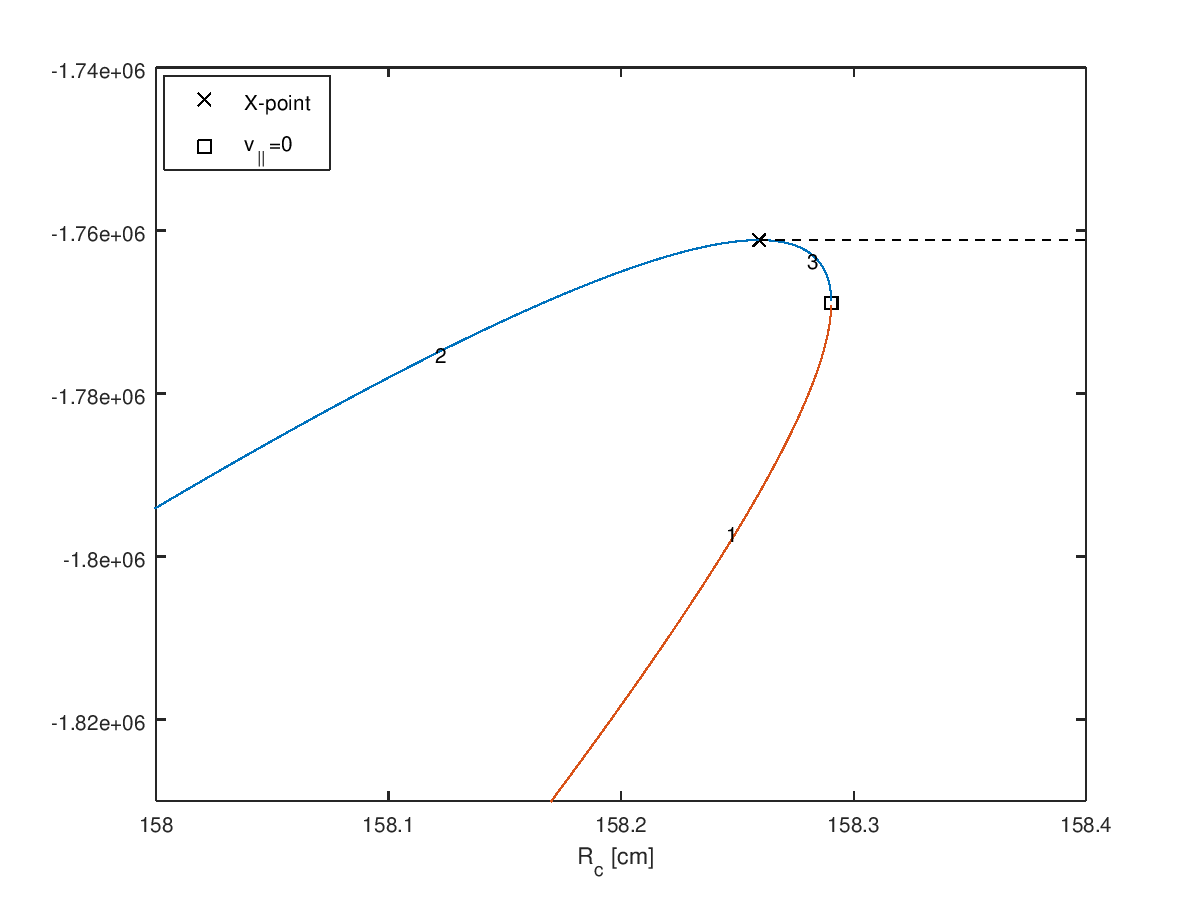
\includegraphics[width=0.4\linewidth]{FIGURES/psiastofRc_X1}
\includegraphics[width=0.4\linewidth]{FIGURES/psiastofRc_X2}
}
\caption[]{
Normalized toroidal moment $\psi^\ast(H_0,J_\perp,\sigma,R_c)$ as function
of Poincar\'e cut parameter $R_c$ for positive ($\sigma=1$, red) and negative
($\sigma=-1$, blue) parallel velocities (upper panel) and zoom around X-points
(lower panel). X-points (x), separatrix crossings (*) and boundaries of allowed 
regions (squares) divide computation domain in 10 classes.
}
\label{fig:psiast}
\end{figure}
An example of separation into classes in case of positive radial electric 
field is shown in Fig.~\ref{fig:psiast}. Here, a ``forbidden'' region
separates the computation domain into two ``allowed'' regions. Left allowed
region contains three classes (one for $\sigma=1$ and two for $\sigma=-1$ 
separated by the X-point). Right allowed region contains seven classes (four
for $\sigma=1$ separated by X-point and two separatrix crossings and three
for $\sigma=-1$ separated by two separatrix crossings). 
Numbers on $\psi^\ast$ curves in Fig.~\ref{fig:psiast} are class indices which
enumerate the classes (zoom into "zoom" plots to see class indices also there).
Domain of $\rho_{pol}$ 
for computation of profiles, $\rho_{pol} \le \sqrt{0.3}$, 
is shown with black solid line. Note that computation domain is wider than 
this domain because it includes footprints of all orbits with 
$\psi^\ast_{min}\le \psi^\ast\le \psi^\ast_{max}$
which may enter $\rho_{pol}$ domain. Here, $\psi^\ast_{min}$ and $\psi^\ast_{max}$
are minimum and maximum values of $\psi^\ast$ attained in the
$\rho_{pol}$ domain with both $\sigma$ values.
\begin{figure}[ht]
\centerline{
\includegraphics[width=0.33\linewidth]{FIGURES/o1}
\includegraphics[width=0.33\linewidth]{FIGURES/o2}
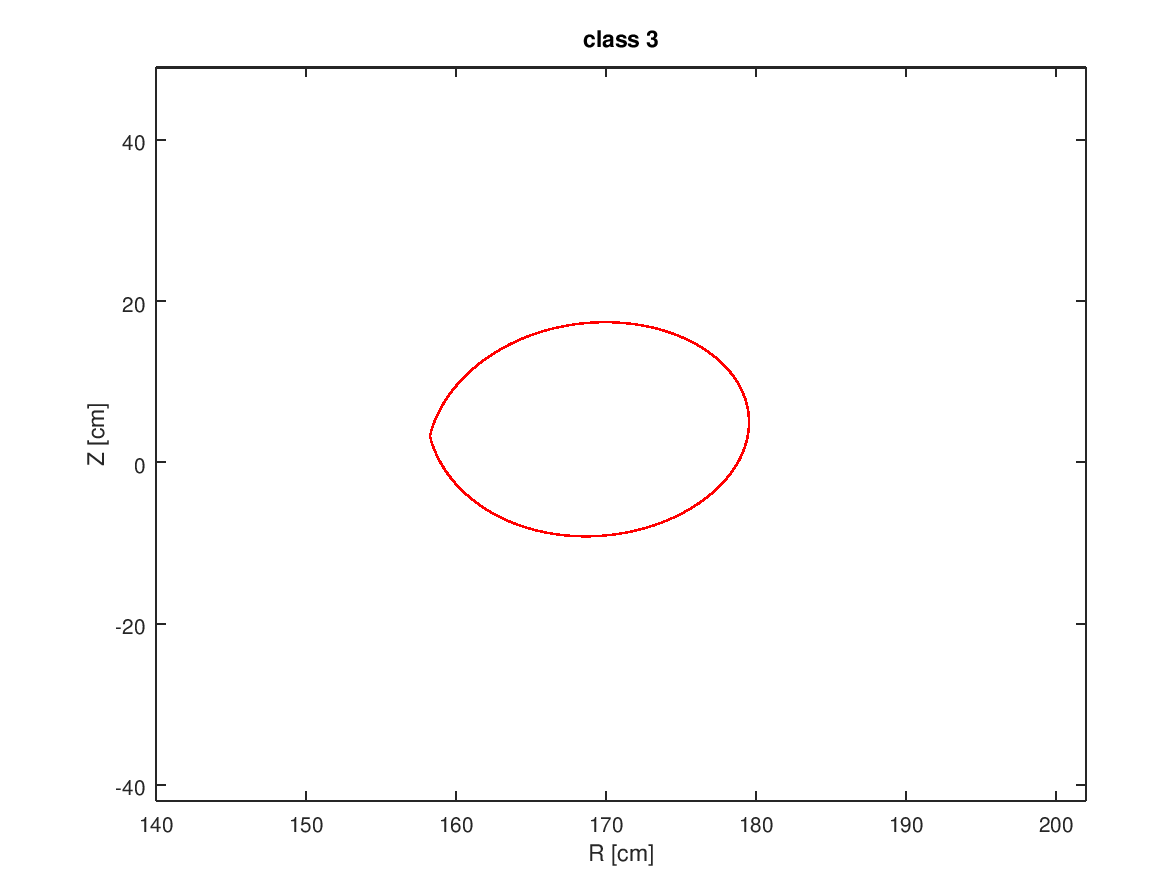
\includegraphics[width=0.33\linewidth]{FIGURES/o3}
}
\centerline{
\includegraphics[width=0.33\linewidth]{FIGURES/o4}
\includegraphics[width=0.33\linewidth]{FIGURES/o5}
\includegraphics[width=0.33\linewidth]{FIGURES/o6}
}
\centerline{
\includegraphics[width=0.33\linewidth]{FIGURES/o7}
\includegraphics[width=0.33\linewidth]{FIGURES/o8}
\includegraphics[width=0.33\linewidth]{FIGURES/o9}
}
\centerline{
\includegraphics[width=0.33\linewidth]{FIGURES/o10}
\includegraphics[width=0.33\linewidth]{FIGURES/oall}
}
\caption[]{
Orbits for 10 classes in Fig.~\ref{fig:psiast}. Class index is indicated
in the titles. Last plot - all classes together (white spot in the middle 
corresponds to the forbidden region with $v_\parallel^2<0$).
}
\label{fig:orbs}
\end{figure}

Orbits for the case of Fig.~\ref{fig:psiast} are plotted in the poloidal 
plane in Fig.~\ref{fig:orbs}. It can be
seen that not all the classes are topologically different. In particular,
classes 1,3,7 belong to the same topological class of outer co-passing particles, 
as well as classes 2,10 (outer counter-passing) and classes 6,9 (trapped).
Therefore, together with class 5 (inner co-passing) and 8 (inner counter-passing)
there are only five topological classes in this case (we call orbits as
``outer'' or ``innter'' if they, respectively, 
do or do not encircle the forbidden region
in the center of configuration). 
For this reason, our classes which belong to the same topological class are
depicted with the same color.  Topological classes are
separated from each other by homoclinic orbits only which is not the case, in
particular, for classes 1,2 (another pair - classes 4,8) which are separated 
by $v_\parallel=0$ point (allowed region boundary).
Moreover, even within a class the same orbit can be present twice with different
values of Poincar\'e cut parameter $R_c$. This is the case if $\psi^\ast$ is 
a non-monotonous function of $R_c$, as for classes 5 and 8, see Fig.~\ref{fig:psiast}.
Therefore, number of orbits (and usually of classes too) in our classification 
is twice the number of topologically different classes. Nevertheless, we pay this
price for the simplicity and robustness of classification algorithm.


Within a class, singularities can be located only at $R_c$ interval boundaries. 
We can 
define four types of boundaries with different behaviour of bounce time for the
following reasons. As a function of $p_\varphi$, 
bounce time has logarithmic singularity for homoclinic orbits
with $p_\varphi=p_\varphi^X$, so that close to those orbits
$\tau_b(p_\varphi) \propto \log|p_\varphi-p_\varphi^X|$.
Besides that, dependence of momentum on cut parameter, $p_\varphi(R_c)$,
has a square root behaviour near reflecting boundaries of allowed regions $R_r$
where $v_\parallel=0$ so that derivative is singular there,
$\partial p_\varphi(R_c)/\partial R_c \propto |R_c-R_r|^{-1/2}$.
Finally, X-points are extremum points of $p_\varphi$ with respect to cut parameter,
so that near these points 
$\partial p_\varphi(R_c)/\partial R_c \propto (R_c-R_X)\rightarrow 0$
in contrast to ``usual'' separatrix crossings where derivative is finite. Therefore,
for $R_X$ and $R_s$ which belong to the same homoclinic orbits one has
$\tau_b(R_c) \approx C_\tau \log|R_c-R_s|$ for ``usual'' crossing and
$\tau_b(R_c) \approx 2 C_\tau \log|R_c-R_X|$ for the X-point where $C_\tau=const$
is the same as for $R_s$.

Thus, the four boundary types are the following:
\begin{itemize}
\item[1] Regular boundary corresponding to maximum $\rho_{pol}$ value. Near this 
boundary, bounce time and its derivatives over cut parameter $R_c$ are finite;
\item[2] Reflecting boundary of allowed region. Near this boundary, derivative
of bounce time over $R_c$ has a square root singularity;
\item[3] ``Usual'' separatrix crossing. Bounce time has a logarithmic singularity;
\item[4] X-point. Bounce time has a logarithmic singularity with a double amplitude.
\end{itemize}
Due to singularities for boundaries 2-4, bounce time cannot be well represented
by a (local) 
polynomial function of $R_c$ in the whole class domain. In order to enable 
such a representation, we introduce new integration variable $x$ such that
$\tau_b(R_c(x))$ can be well represented by a polynomial of $x$ in the whole domain.
For example, logarithmic singularity turns into linear dependence of new variable
for variable change $R_c(x) = R_X + \Delta R \exp(x)$ so that
$\tau_b \propto \log|R_c-R_X| \propto x$ with $x\rightarrow - \infty$.
Therefore, bounce time can be well represented by polynomial interpolation for
$x>x_{min}$ where $|x_{min}|$ is large but finite, and by linear extrapolation
for $x<x_{min}$.

For treatment of 16 interval types (4 variants for each boundary) we introduce 9 types
of variable change as follows,
\be{convreg}
R_c=R_c(x)=R^{[min]}_k+\left(R^{[max]}_k-R^{[min]}_k\right) \xi_{i_k j_k}(x),
\ee
where $\xi_{ij}(x)$ are monotonous class parameterization 
functions changing in the limits $0<\xi_{ij}<1$
with indices $i$ and $j$ denoting types of left and right boundary, respectively.
Boundary types 3 and 4 are indistinguishable for functions $\xi_{ij}$ 
so that $\xi_{i4}=\xi_{i3}$ and $\xi_{4j}=\xi_{3j}$, but they
are taken into account in the range of independent variable $x$ where interpolation
is used (in the rest of $x$ range, extrapolation is used). These functions are
\be{xifuns}
\begin{array}{lc}
\xi_{11}(x) = x,                     &\qquad  0\le x \le 1, \\
\xi_{12}(x) = 1-(1-x)^2,             &\qquad  0\le x \le 1, \\  
\xi_{13}(x) = \xi_{14}(x) =\tanh(x), &\qquad  0\le x \le \infty, \\  
\xi_{21}(x) = x^2,                   &\qquad  0\le x \le 1, \\
\xi_{22}(x) = \frac{1}{2}\left(1-\cos(\pi x)\right) 
                                     &\qquad  0\le x \le 1, \\
\xi_{23}(x) = \xi_{24}(x) =\tanh^2(x), &\qquad  0\le x \le \infty, \\  
\xi_{31}(x) = \xi_{41}(x) =\tanh(x)+1, &\qquad  -\infty \le x \le 0, \\  
\xi_{32}(x) = \xi_{42}(x) =1-\tanh^2(x), &\qquad  -\infty \le x \le 0, \\  
\xi_{33}(x) = \xi_{34}(x) = \xi_{43}(x) = \xi_{44}(x) 
=\frac{1}{2}\left(1+\tanh(x)\right), &\qquad  -\infty \le x \le \infty. \\  
\end{array}
\ee
Ranges of independent variable $x$ used for interpolation do not coincide in all
cases with ranges indicated in~\eq{xifuns}. Namely, these ranges for
all possible interval types are the following,
\begin{itemize}
\item[11:] $\qquad 0\le x \le 1$,
\item[12:] $\qquad 0\le x \le 1-\varepsilon$,
\item[13:] $\qquad 0\le x \le -\log\left(\frac{\varepsilon}{\delta}\right)$,
\item[14:] $\qquad 0\le x 
\le -\frac{1}{2}\log\left(\frac{\varepsilon}{\delta}\right)$,
\item[21:] $\qquad \varepsilon \le x \le 1$,
\item[22:] $\qquad \varepsilon \le x \le 1-\varepsilon$,
\item[23:] $\qquad \varepsilon \le x 
\le -\log\left(\frac{\varepsilon}{\delta}\right)$,
\item[24:] $\qquad \varepsilon \le x 
\le -\frac{1}{2}\log\left(\frac{\varepsilon}{\delta}\right)$,
\item[31:] $\qquad \log\left(\frac{\varepsilon}{\delta}\right) \le x \le 0$,
\item[32:] $\qquad \log\left(\frac{\varepsilon}{\delta}\right) 
\le x \le -\varepsilon$,
\item[33:] $\qquad \log\left(\frac{\varepsilon}{\delta}\right) \le x 
\le -\log\left(\frac{\varepsilon}{\delta}\right)$,
\item[34:] $\qquad \log\left(\frac{\varepsilon}{\delta}\right) \le x 
\le -\frac{1}{2}\log\left(\frac{\varepsilon}{\delta}\right)$,
\item[41:] $\qquad \frac{1}{2}\log\left(\frac{\varepsilon}{\delta}\right) \le x \le 0$,
\item[42:] $\qquad \frac{1}{2}\log\left(\frac{\varepsilon}{\delta}\right) 
\le x \le -\varepsilon$,
\item[43:] $\qquad \frac{1}{2}\log\left(\frac{\varepsilon}{\delta}\right) \le x 
\le -\log\left(\frac{\varepsilon}{\delta}\right)$,
\item[44:] $\qquad \frac{1}{2}\log\left(\frac{\varepsilon}{\delta}\right) \le x 
\le -\frac{1}{2}\log\left(\frac{\varepsilon}{\delta}\right)$,
\end{itemize}
where $\varepsilon \ll 1$ is accuracy parameter and 
$\delta = \left|R^{[max]}_k-R^{[min]}_k\right|/R^{[min]}_k$ is the relative width
of the class domain. Results of adaptive polynomial interpolation of bounce time
and toroidal displacement per bounce time are shown for the cases of 
Figs.~\ref{fig:psiast} and~\ref{fig:orbs} in Section~\ref{ssec:adaptive}.

In the following, we denote class domain boundaries indicated in~\eq{xifuns}
as follows, $x^{[min]}_k \le x \le x^{[max]}_k$, i.e. directly, without mentioning
boundary types. 
Thus, integral~\eq{finalint_withlims_taub} is
\be{finalint_over_classes}
A=2\pi^2 
\int\limits_{e_\alpha\Phi_{\rm min}}^\infty \rd H_0
\int\limits_0^{J_\perp^{\rm max}(H_0)} \rd J_\perp
\sum\limits_{k=1}^{N_{\rm cl}}
\int\limits_{x^{[min]}_k}^{x^{[max]}_k} \rd x
\left|\difp{p_\varphi}{x}\right|
\int\limits_0^{\tau_b} \rd \tau\;
\cA\;
\Theta\left(r_0-r\right),
\ee
where~\eq{convreg} is used in 
$r=r\left({\cal R}(R_c(x),\tau), {\cal Z}(R_c(x),\tau)\right)$ and in
$$
\difp{p_\varphi}{x}=\difp{p_\varphi}{R_c}\difp{R_c}{x}.
$$

We are interested in two kinds of integrals. First one is integrals~\eq{bj0}
of the equilibrium quantities. They correspond to the following subintegrand,
\be{bisubint}
\cA(R,Z)=\phi_i(r(R,Z)) a_0 f_0 \Theta_w(r_a-r(R,Z)),
\ee
and explicitly are 
\be{bi_classes}
b_i=2\pi^2
\int\limits_{e_\alpha\Phi_{\rm min}}^\infty \rd H_0
\int\limits_0^{J_\perp^{\rm max}(H_0)} \rd J_\perp
\sum\limits_{k=1}^{N_{\rm cl}}
\int\limits_{x^{[min]}_k}^{x^{[max]}_k} \rd x
\left|\difp{p_\varphi}{x}\right| f_0
\int\limits_0^{\tau_b} \rd \tau\;
a_0\; \phi_i(r)
\Theta_w\left(r_a-r\right),
\ee
where we omitted the arguments in the subintegrands, in particular
of $a_0$ and $r$ which depend on orbit parameter $\tau$. Box 
averages~\eq{Abox_0_noncan} are a particular case of~\eq{bi_classes},
\be{boxav_classes}
A_{0\rm box}(r_a)=\left.b_i\right|_{\phi_i=1},
\ee
which can be seen from the comparison of~\eq{bisubint} with~\eq{boxmaxwint}.

Second integral of interest
is the radial particle flux density
integrated over the volume, Eq.~\eq{boxflux},
which takes the form
\bea{boxflux_classes}
\Gamma_{\rm box}(r_0) &=& 
-\pi^3\sum_\bm 
\int\limits_{e_\alpha\Phi_{\rm min}}^\infty \rd H_0
\int\limits_0^{J_\perp^{\rm max}(H_0)} \rd J_\perp
\sum\limits_{k=1}^{N_{\rm cl}}
\int\limits_{x^{[min]}_k}^{x^{[max]}_k} \rd x
\left|\difp{p_\varphi}{x}\right| 
%\int \rd H_0\int\rd J_\perp\int\rd p_\varphi
\;\left|H_{\bm}\right|^2\delta(m_2\omega_b+m_3\Omega_\varphi)\;
\nonumber \\
&\times&
\left(m_2\omega_b\difp{f_0}{H_0}+m_3\difp{f_0}{p_\varphi}\right)
\int\limits_0^{\tau_b}\rd \tau\;
\left(
m_2\omega_b\left(\difp{r}{H_0}\right)_{p_\varphi,\theta^2}
+m_3\left(\difp{r}{p_\varphi}\right)_{\theta^2}
\right)\Theta(r_0-r),
\eea
where we omitted dependence of $r$ on phase space coordinates.
In this expression it is more convenient to express canonical
frequencies via bounce time $\tau_b$ and toroidal displacement
over bounce time $\Delta\varphi_b$ since these are the quantities
directly computed by the orbit solver and then sampled by adaptive
grid formation algorithm over class parameter $x$. Namely,
using
\be{canfreqs}
\omega_b=\frac{2\pi}{\tau_b},
\qquad
\Omega_\varphi=\frac{\Delta\varphi_b}{\tau_b},
\ee
we get using the properties of $\delta$-function
\bea{boxflux_classes_conv}
\Gamma_{\rm box}(r_0) &=&
-\pi^3\sum_\bm |m_3|
\int\limits_{e_\alpha\Phi_{\rm min}}^\infty \rd H_0
\int\limits_0^{J_\perp^{\rm max}(H_0)} \rd J_\perp
\sum\limits_{k=1}^{N_{\rm cl}}
\int\limits_{x^{[min]}_k}^{x^{[max]}_k} \rd x
\left|\difp{p_\varphi}{x}\right|
\;\left|H_{\bm}\right|^2
\delta\left(\Delta\varphi_b+\frac{2\pi m_2}{m_3}\right)\;
\nonumber \\
&\times&
\left(
\tau_b\difp{f_0}{p_\varphi}
-\Delta\varphi_b\difp{f_0}{H_0}
\right)
\left\langle
\left(
\tau_b\left(\difp{r}{p_\varphi}\right)_{p_\varphi,\theta^2}    
-\Delta\varphi_b\left(\difp{r}{H_0}\right)_{\theta^2}
\right)\Theta(r_0-r)
\right\rangle_b,
\eea
where angular brackets in the last term stand for the bounce average,
\be{boubox}
\left\langle
F
\right\rangle_b
=
\frac{1}{\tau_b}
\int\limits_0^{\tau_b}\rd \tau\;
F =\frac{1}{2\pi}\int\limits_0^{2\pi} \rd \theta^2 F.
\ee
Using the following representation of Heaviside function,
\be{reprTheta}
\Theta(x)=\frac{1}{2}\frac{\rd}{\rd x}(x+|x|),
\ee
we can present bounce average in~\eq{boxflux_classes_conv} as
\bea{bouav_theta}
\left\langle
\left(
\tau_b\left(\difp{r}{p_\varphi}\right)_{\theta^2}
-\Delta\varphi_b\left(\difp{r}{H_0}\right)_{p_\varphi,\theta^2}
\right)\Theta(r_0-r)
\right\rangle_b
&=&
\frac{1}{2}
\left(
\tau_b\difp{}{p_\varphi}-\Delta\varphi_b\left(\difp{}{H_0}\right)_{p_\varphi}
\right)
\nonumber \\
&\times&
\left\langle
r_0-r+|r_0-r|
\right\rangle_b,
\eea
which can be more convenient for the numerics. Here, the derivative for constant
$p_\varphi$ is expressed via derivative for constant $x$ as follows
\be{derH0_pp}
\left(\difp{}{H_0}\right)_{p_\varphi}
=
\left(\difp{}{H_0}\right)_{x}-\left(\difp{p_\varphi}{H_0}\right)_x
\left(\difp{p_\varphi}{x}\right)^{-1}\difp{}{x}
=
\left(\difp{}{H_0}\right)_{x}-\frac{h_\varphi}{v_\parallel}
\left(\difp{p_\varphi}{x}\right)^{-1}\difp{}{x},
\ee
so that~\eq{bouav_theta} is expressed via derivative over $H_0$ for constant $x$
as
\bea{bouav_theta_cx}
\left\langle
\dots
\right\rangle_b
&=&
\frac{1}{2}
\left(
\left(\tau_b-\frac{h_\varphi}{v_\parallel}\right)
\left(\difp{p_\varphi}{x}\right)^{-1}\difp{}{x}
-\Delta\varphi_b\left(\difp{}{H_0}\right)_{x}
\right)
\left\langle
r_0-r+|r_0-r|
\right\rangle_b,
\eea
where $h_\varphi=B_\varphi/B$ and $v_\parallel$ are evaluated at the Poincar\'e cut.

It should be noted that up to this point 
a particular form~\eq{equilmaxw} of the unperturbed
distribution function $f_0=f_0(\psi^\ast,H_0,J_\perp,\sigma)$ 
has not been used in~\eq{bi_classes} and~\eq{boxflux_classes_conv}.
Therefore, a Maxwellian-like distribution~\eq{equilmaxw} which well approximates
equilibrium distribution function in case of constant temperature and mild density
and electrostatic potential gradients can be replaced by a distribution function
from some 3D neoclassical solver for the long mean free path regime in case it
is available. In the next section we will already use our particular 
form~\eq{equilmaxw}.


\section{Normalized variables, numerics, tests}

\noindent
In the orbit integrator, time and momenta are used in the normalized form
\be{normvar}
\hat t = v_0 t,
\qquad
\hat \bp = \bp / p_0,
\qquad
\ee
where $p_0 = m_\alpha v_0$ is a reference momentum defined for species $\alpha$
via some reference kinetic energy ${\cal E}_{\rm ref}$ as $p_0 = \sqrt{2 m_\alpha {\cal E}_{\rm ref}}$. Electrostatic potential and Hamiltonian are normalized as
\be{normPhiandH}
\hat\Phi=e_\alpha\Phi/{\cal E}_{\rm ref},
\qquad
\hat H_0 = H_0/{\cal E}_{\rm ref} = \hat p^2 + \hat\Phi.
\ee
Finally, we use $\psi^\ast$ instead of $p_\varphi$ (see~\eq{psiast}) and use the
normalized perpendicular invariant
\be{normjperp}
\hat J_\perp = \frac{\hat p_\perp^2}{B}=\frac{e_\alpha J_\perp}{m_\alpha c{\cal E}_{\rm ref}}.
\ee
In these variables, integrals~\eq{bi_classes} with substitution of~\eq{equilmaxw}
take the form
\bea{bi_classes_norm}
b_i &=& \frac{\sqrt{\pi}}{2}
\int\limits_{\hat\Phi_{\rm min}}^\infty \rd \hat H_0
\int\limits_0^{\hat J_\perp^{\rm max}(\hat H_0)} \rd \hat J_\perp
\sum\limits_{k=1}^{N_{\rm cl}}
\int\limits_{x^{[min]}_k}^{x^{[max]}_k} \rd x
\left|\difp{\psi^\ast}{x}\right| 
\nonumber \\
&\times&
\frac{\bar n_\alpha(\psi^\ast)}{\hat T_\alpha^{3/2}(\psi^\ast)}
\exp\left(\frac{\hat \Phi(\psi^\ast)-\hat H_0}{\hat T_\alpha(\psi^\ast)} \right)
\int\limits_0^{\hat \tau_b} \rd \hat \tau\;
a_0\; \phi_i(r)
\Theta_w\left(r_a-r\right),
\eea
where
\be{That}
\hat T_\alpha = \frac{T_\alpha}{{\cal E}_{\rm ref}}.
\ee
which is even simpler in case of constant temperature and 
${\cal E}_{\rm ref}=T_\alpha$ where $\hat T_\alpha=1$.
%\bea{bi_classes_norm_tconst}
%b_i &=& \frac{\sqrt{\pi}}{2}
%\int\limits_{\hat\Phi_{\rm min}}^\infty \rd \hat H_0
%\int\limits_0^{\hat J_\perp^{\rm max}(\hat H_0)} \rd \hat J_\perp
%\sum\limits_{k=1}^{N_{\rm cl}}
%\int\limits_{x^{[min]}_k}^{x^{[max]}_k} \rd x
%\left|\difp{\psi^\ast}{x}\right| 
%\nonumber \\
%&\times&
%\bar n_\alpha(\psi^\ast)
%\exp\left(-\left(\hat H_0-\hat \Phi(\psi^\ast)\right)\right)
%\int\limits_0^{\hat \tau_b} \rd \hat \tau\;
%a_0\; \phi_i(r)
%\Theta_w\left(r_a-r\right),
%\eea

\subsection{Check for the paraxial region}

Let us check the validity of this expression for particle 
density, $a_0=1$, in the paraxial region
of circular tokamak in zero Larmor radius limit and without radial electric field. 
We replace $\Theta_w$ with usual $\Theta$, 
fix $r$ to minor radius of quasi-toroidal coordinates,
and can approximately write
$$
\frac{\rd V(r)}{\rd r} \approx 4\pi^2 R_0 r,
\qquad
\langle A \rangle \approx n_\alpha(r),
$$
so that Eq.~\eq{coefsset} results in
\be{thesame}
b_i \approx 4\pi^2 R_0 \int\limits_0^{r_a}\rd r\, r\, n_\alpha(r)\phi_i(r).
\ee
We use
$$
\difp{\psi^\ast}{r} \approx \difp{\psi}{r} \approx \frac{r B_0}{q_0}
$$
were 0 stands for axial values, ignore trapped particles so that there are only
two classes (co- and counter-passing) with constant parallel velocities such that
$$
\hat \tau_b \approx \frac{2\pi q_0R_0 }{|\hat p_\parallel|}
=\frac{2\pi q_0R_0}{\sqrt{\hat H_0 -\hat J_\perp B_0}}.
$$
Since $r$ is constant along the orbits we get for~\eq{bi_classes_norm}
\bea{bi_check}
b_i &=& \sqrt{\pi}
\int\limits_{0}^\infty \rd \hat H_0
\int\limits_0^{\hat H_0/B_0} \rd \hat J_\perp
\int\limits_{x^{[min]}_k}^{x^{[max]}_k} \rd x
\left|\difp{\psi^\ast}{x}\right|
\bar n_\alpha \phi_i(r) \Theta\left(r_a-r\right)
\exp\left(-\hat H_0\right)
\hat \tau_b
\nonumber \\
&=&
2\sqrt{\pi}
\int\limits_{0}^\infty \rd \hat H_0
\int\limits_0^{\hat H_0/B_0} \rd \hat J_\perp
\int\limits_0^{r_a} \rd r
\left|\difp{\psi^\ast}{r}\right|
\bar n_\alpha \phi_i(r)
\exp\left(-\hat H_0\right)
\hat \tau_b
\nonumber \\
&=&
4\pi^{3/2}R_0B_0
\int\limits_{0}^\infty \rd \hat H_0
\int\limits_0^{\hat H_0/B_0} \rd \hat J_\perp
\int\limits_0^{r_a} \rd r
\bar n_\alpha \phi_i(r) 
\exp\left(-\hat H_0\right)
\frac{r}
{\sqrt{\hat H_0 -\hat J_\perp B_0}}
\nonumber \\
&=&
8\pi^{3/2}R_0
\int\limits_{0}^\infty \rd \hat H_0
\sqrt{\hat H_0}
\int\limits_0^{r_a} \rd r \;r
\bar n_\alpha \phi_i(r)
\exp\left(-\hat H_0\right)
\nonumber \\
&=&
4\pi^2R_0
\int\limits_0^{r_a} \rd r \,r\,
\bar n_\alpha \phi_i(r),
\eea
i.e. we get the same as~\eq{thesame}.

\subsection{Adaptive grid sampling over class parameter}
\label{ssec:adaptive}

Adaptive grid over class parameter $x$ is created by binary refinement of the initial
equidistant grid which consists of a single stencil (set of points required for
Lagrange interpolation of a given order). For the refinement, difference between
interpolations of bounce time, toroidal displacement and bounce integrals using
stencils shifted by one position with respect to each other 
is checked for each grid interval and, if this difference for any interpolated 
quantity relative to this quantity exceed the required interpolation error interval
is split into two. Procedure is repeated until the required accuracy is reached.

Results of this refinement for the case of Figs.~\ref{fig:psiast} 
and~\ref{fig:orbs} are shown for the normalized bounce time
$\hat \tau_b = v_0 \tau_b$ in Figs.~\ref{fig:taub} and~\ref{fig:taub_x},
and for the toroidal displacement per bounce time $\Delta\varphi_b$ 
in Figs~\ref{fig:delphi} and~\ref{fig:delphi_x}. Note that the orbits shown
in Fig.~\ref{fig:orbs} correspond to grid nodes of the adaptive interpolation
grid in Figs.~\ref{fig:taub}-\ref{fig:delphi_x}. 
%
\begin{figure}[ht]
\centerline{
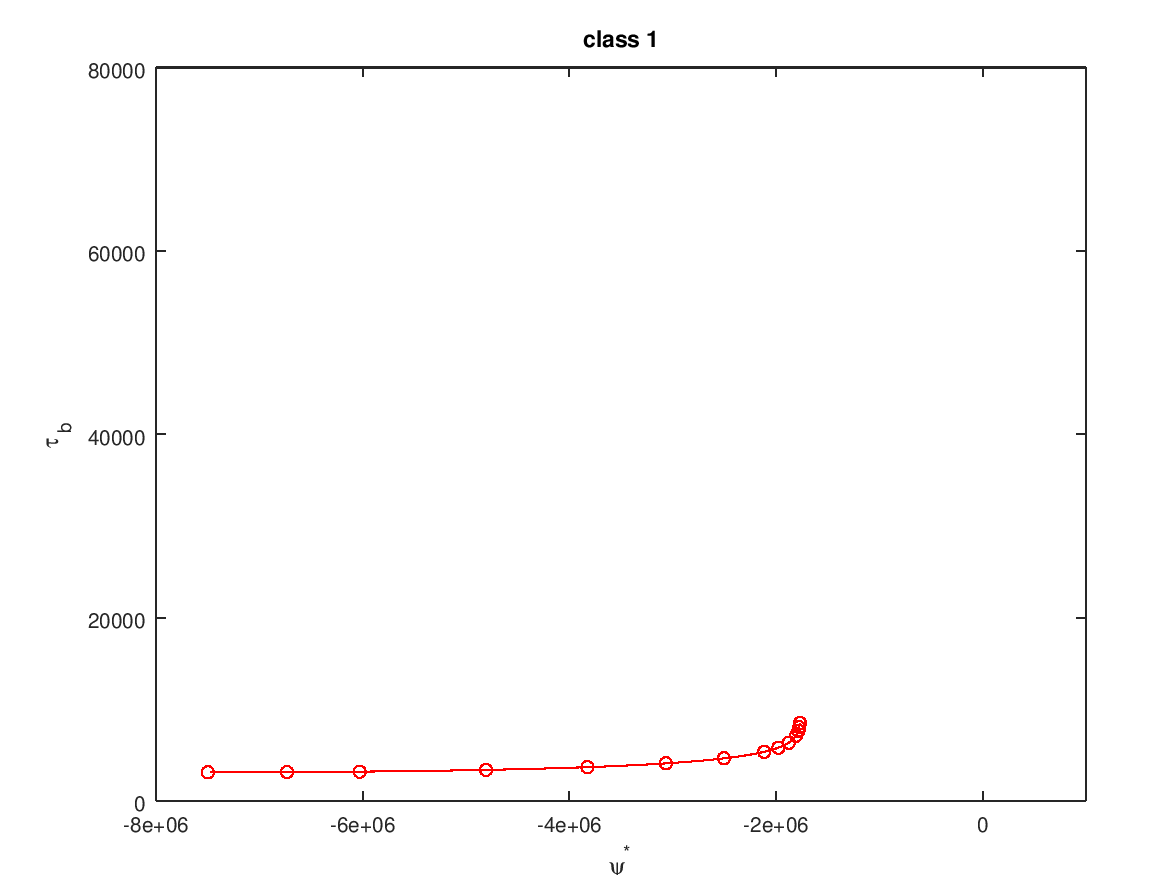
\includegraphics[width=0.33\linewidth]{FIGURES/taub1}
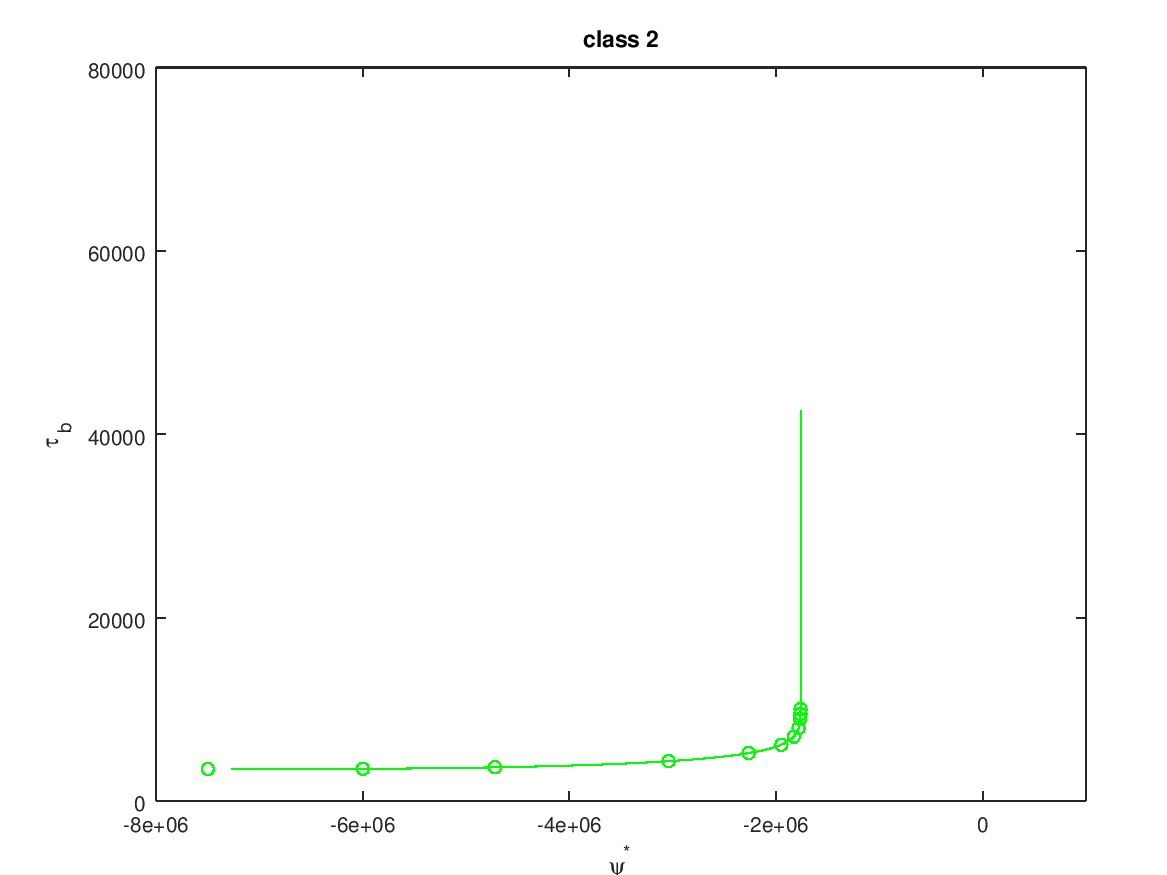
\includegraphics[width=0.33\linewidth]{FIGURES/taub2}
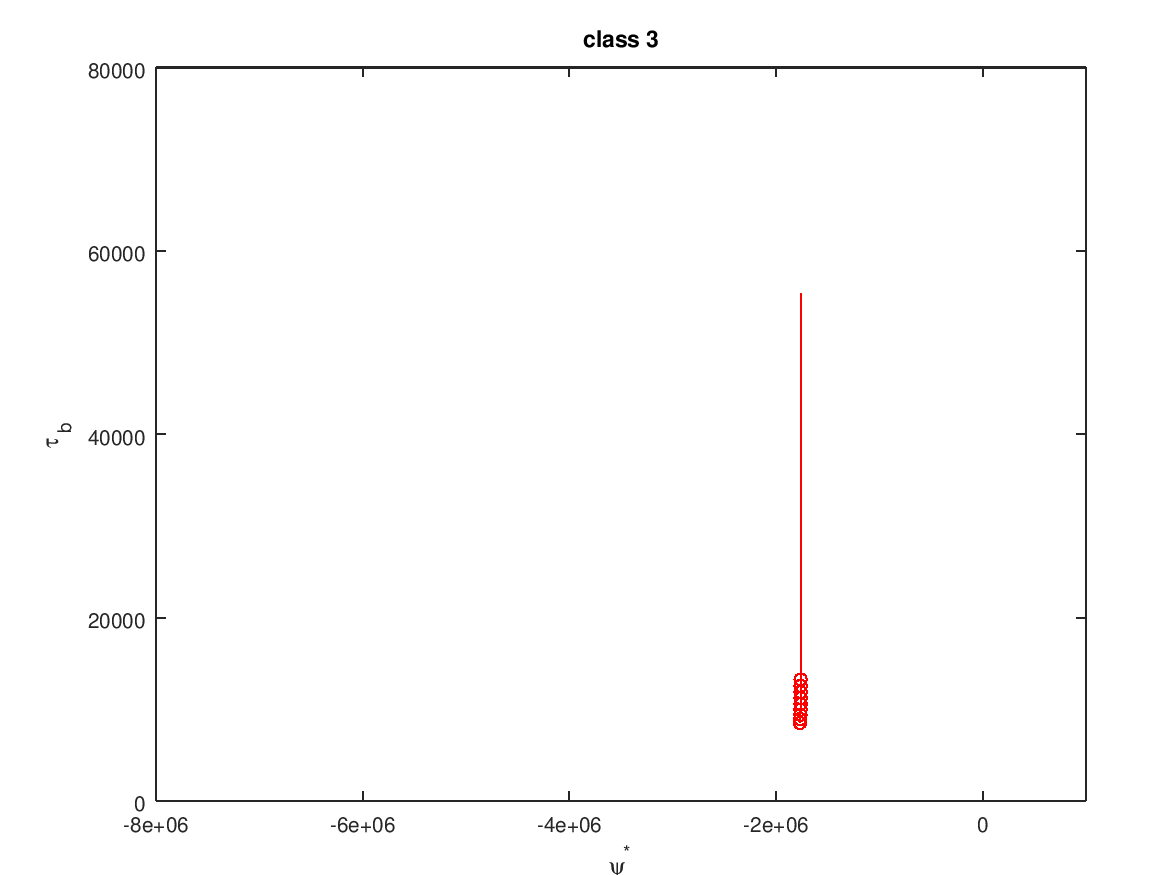
\includegraphics[width=0.33\linewidth]{FIGURES/taub3}
}
\centerline{
\includegraphics[width=0.33\linewidth]{FIGURES/taub4}
\includegraphics[width=0.33\linewidth]{FIGURES/taub5}
\includegraphics[width=0.33\linewidth]{FIGURES/taub6}
}
\centerline{
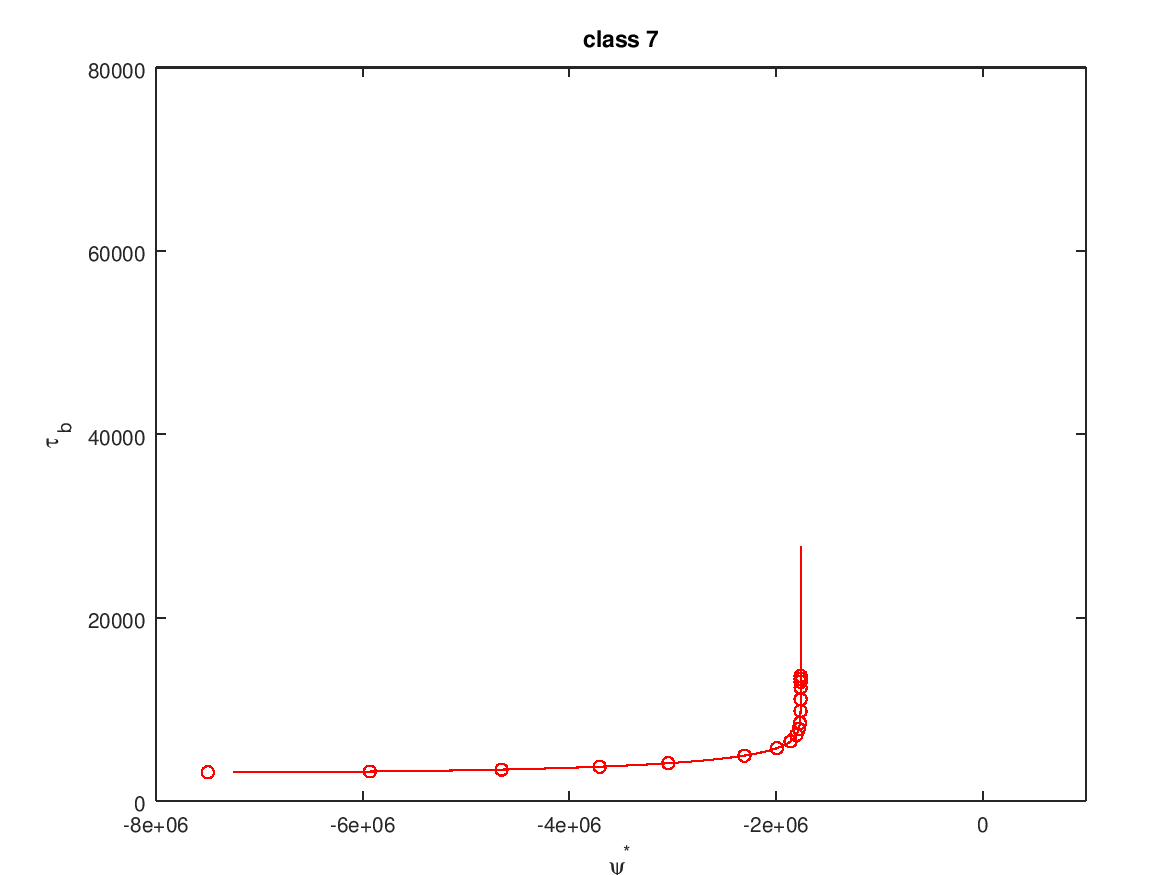
\includegraphics[width=0.33\linewidth]{FIGURES/taub7}
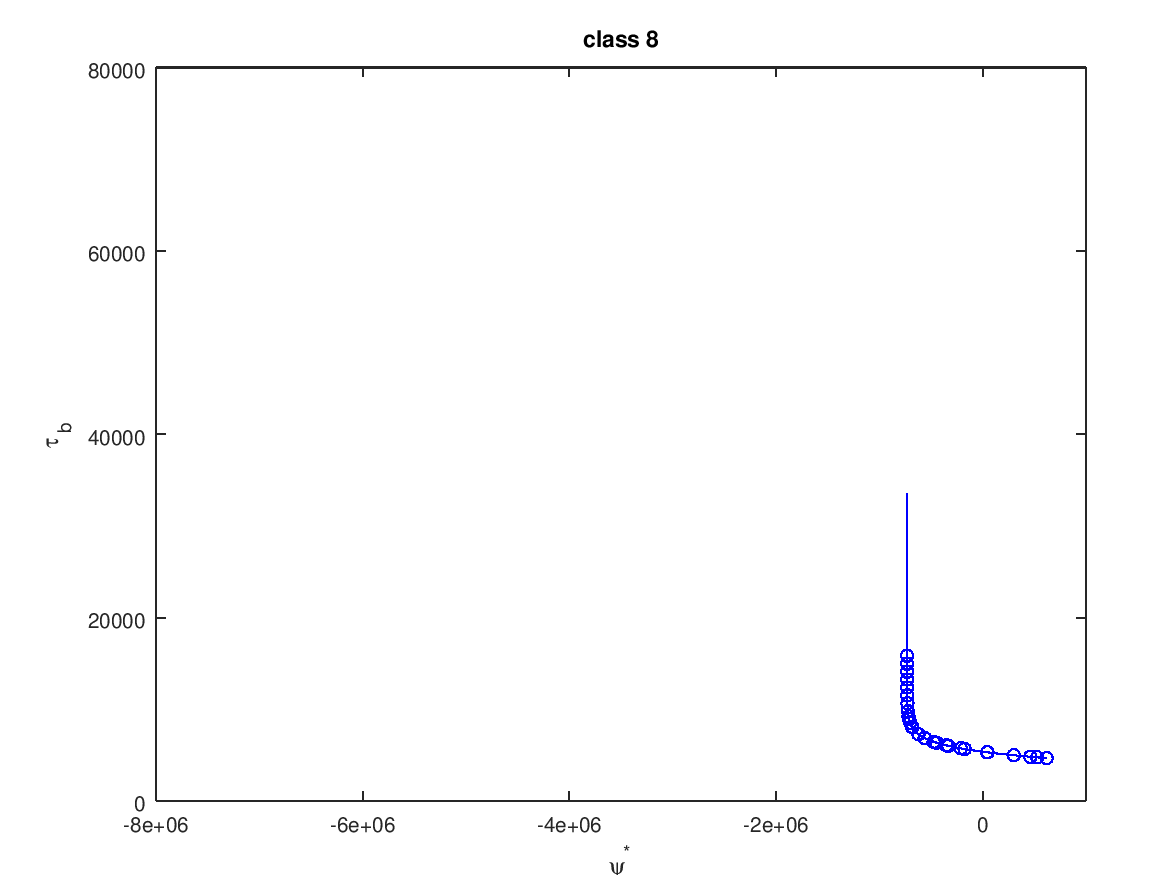
\includegraphics[width=0.33\linewidth]{FIGURES/taub8}
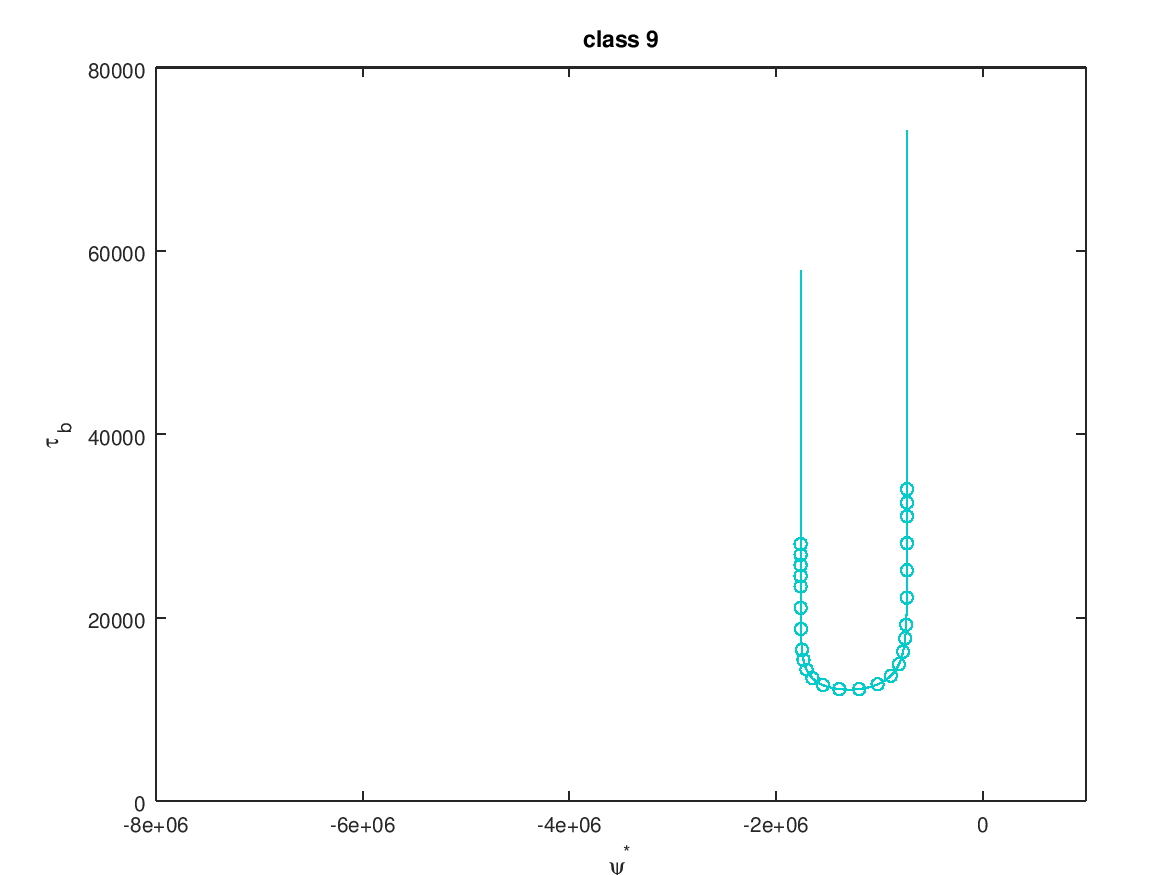
\includegraphics[width=0.33\linewidth]{FIGURES/taub9}
}
\centerline{
\includegraphics[width=0.33\linewidth]{FIGURES/taub10}
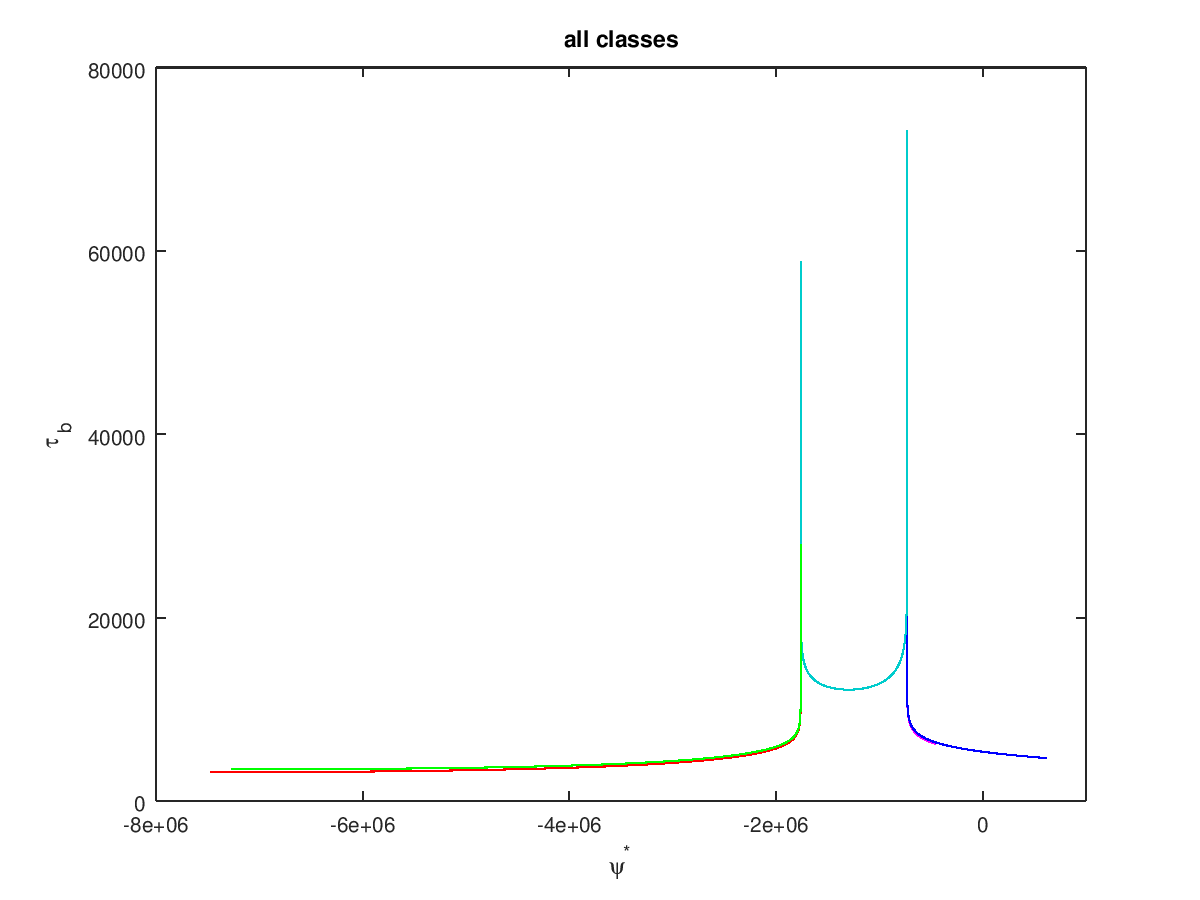
\includegraphics[width=0.33\linewidth]{FIGURES/taub_all}
}
\caption[]{
Normalized bounce time $\hat\tau_b$ as function of $\psi^\ast$ for 10 classes 
in Figs.~\ref{fig:psiast} and~\ref{fig:orbs}. Class index is indicated
in the titles,  last plot - all classes together.
Color coding is the same as in Fig.~\ref{fig:orbs}. Solid - 
interpolation, markers - adaptive grid points.
}
\label{fig:taub}
\end{figure}
%
For the formation of adaptive grid, polynomials of 6-th order have been
used with required relative error $10^{-3}$.
As seen from Figs.~\ref{fig:taub_x} and~\ref{fig:delphi_x}, adaptive grid
in $x$ variable well resolves the interpolated quantities. 
In the regions where solid lines solid lines are without markers depicting
the interpolation grid, linear extrapolation is used.
%
\begin{figure}[ht]
\centerline{
\includegraphics[width=0.33\linewidth]{FIGURES/taub_x1}
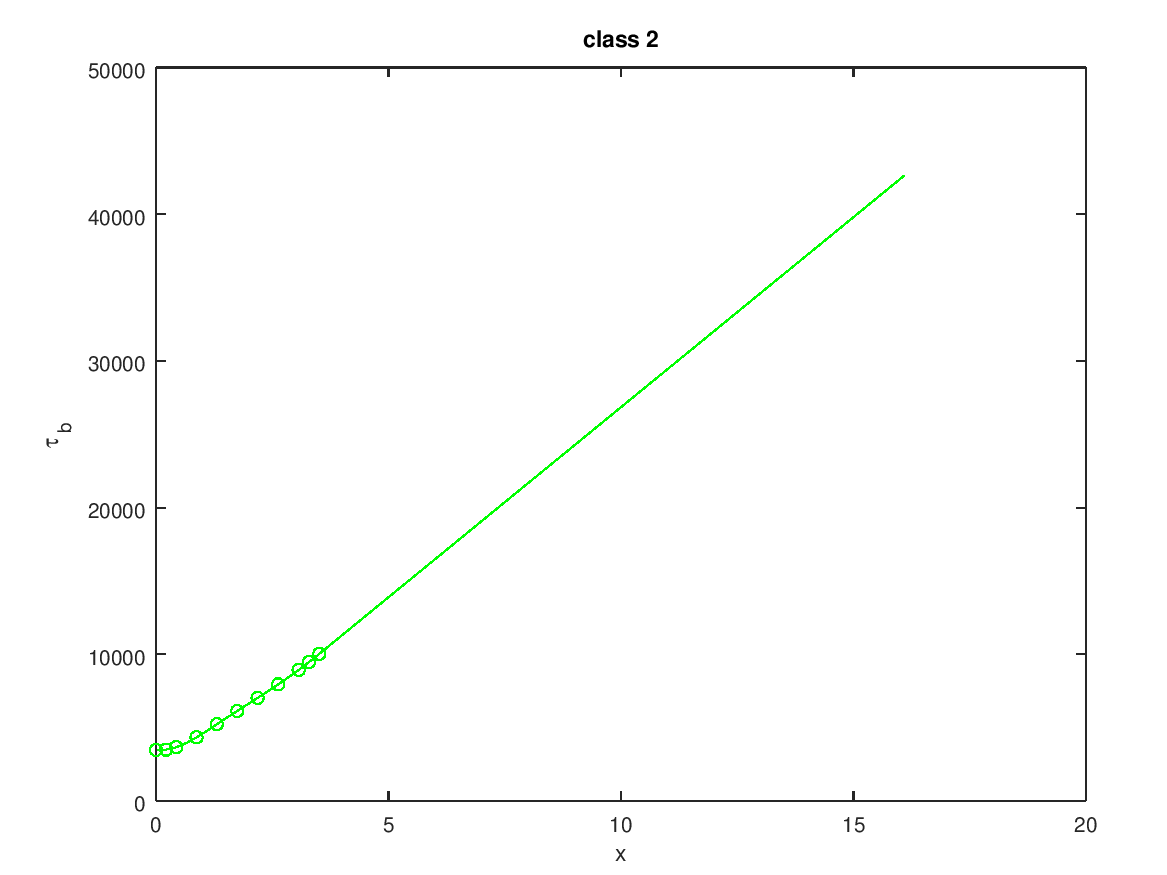
\includegraphics[width=0.33\linewidth]{FIGURES/taub_x2}
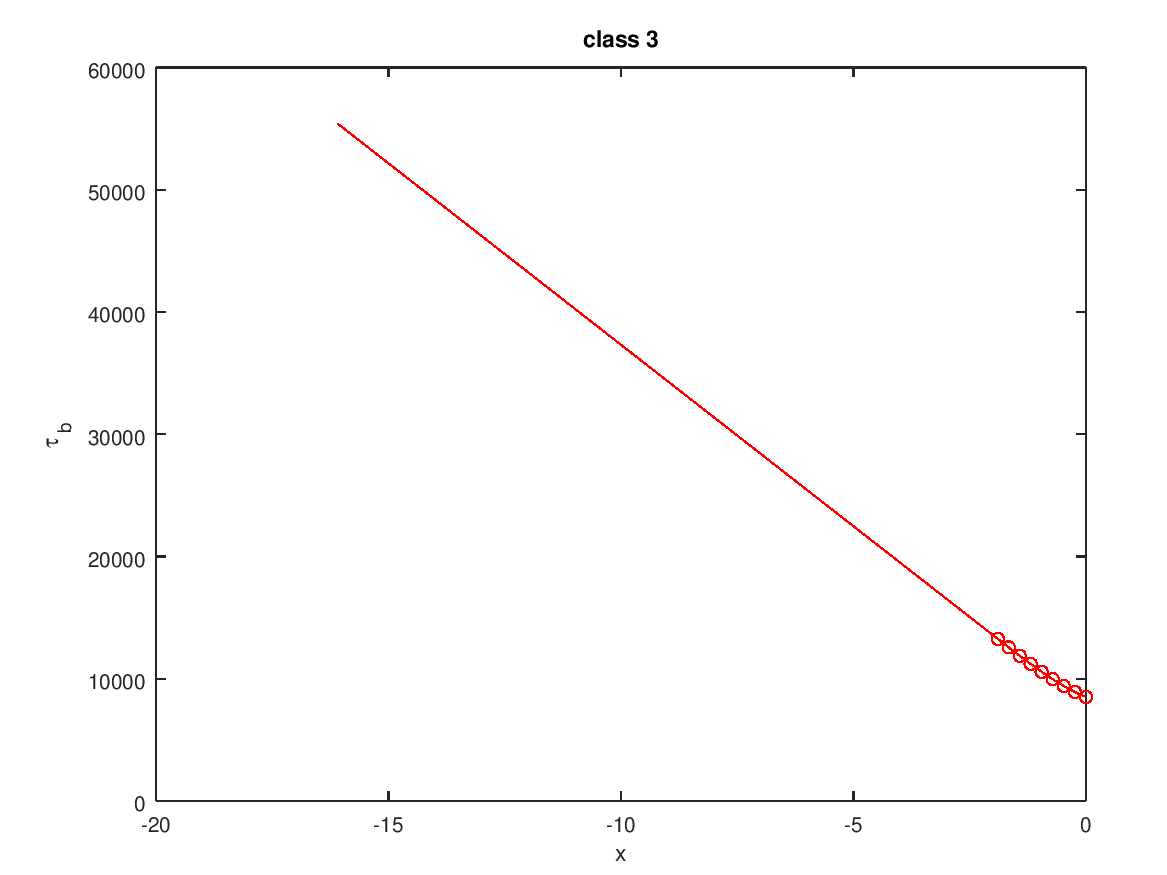
\includegraphics[width=0.33\linewidth]{FIGURES/taub_x3}
}
\centerline{
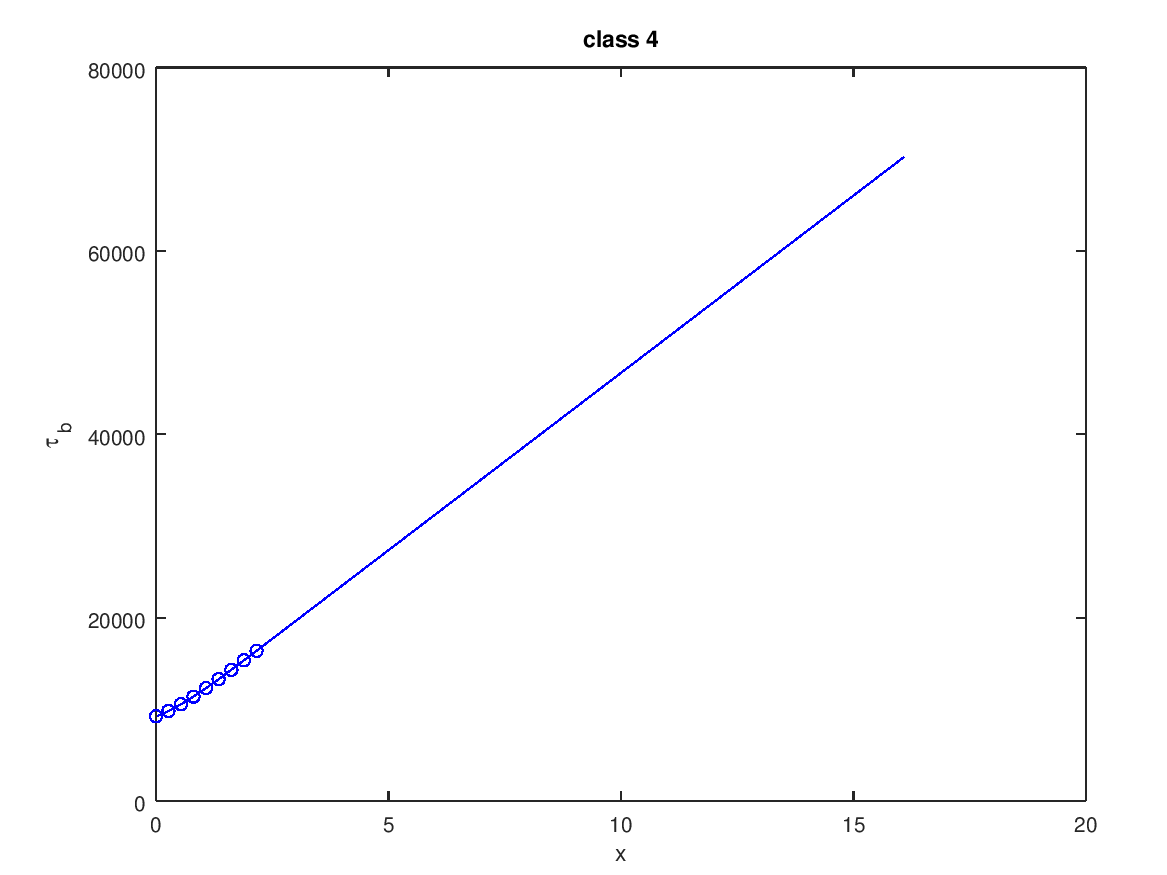
\includegraphics[width=0.33\linewidth]{FIGURES/taub_x4}
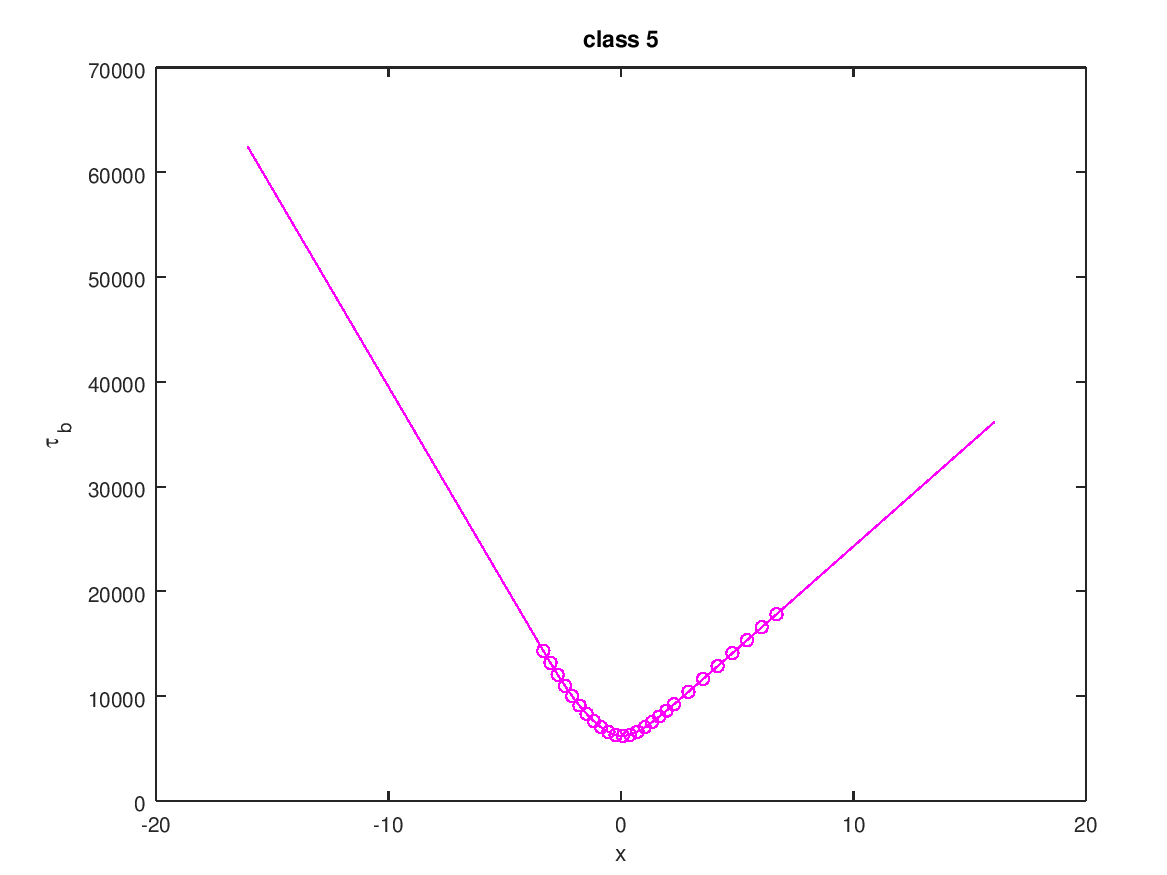
\includegraphics[width=0.33\linewidth]{FIGURES/taub_x5}
\includegraphics[width=0.33\linewidth]{FIGURES/taub_x6}
}
\centerline{
\includegraphics[width=0.33\linewidth]{FIGURES/taub_x7}
\includegraphics[width=0.33\linewidth]{FIGURES/taub_x8}
\includegraphics[width=0.33\linewidth]{FIGURES/taub_x9}
}
\centerline{
\includegraphics[width=0.33\linewidth]{FIGURES/taub_x10}
}
\caption[]{
Normalized bounce time $\hat\tau_b$ as function of class parameter $x$ 
for 10 classes in Fig.~\ref{fig:taub}. Class indices, color coding and
line styles - the same as in Fig.~\ref{fig:taub}.
}
\label{fig:taub_x}
\end{figure}
%

It can be seen, in particular, from the last plots in Figs~\ref{fig:taub}
and~\ref{fig:delphi} that our classes are indistinguishable, i.e. their bounce 
time and displacement match continuously with continuous derivatives,
as long as they belong to the same topological class.
%
\begin{figure}[ht]
\centerline{
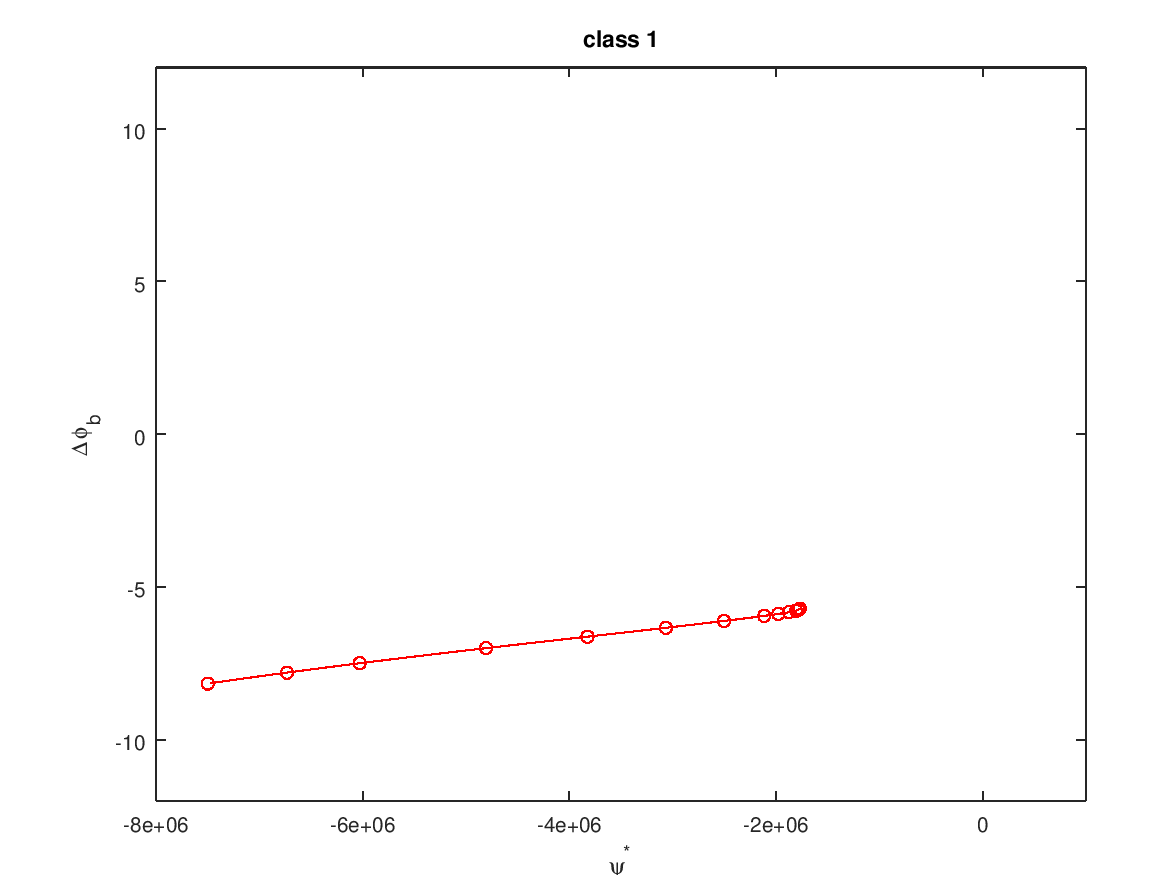
\includegraphics[width=0.33\linewidth]{FIGURES/delphi1}
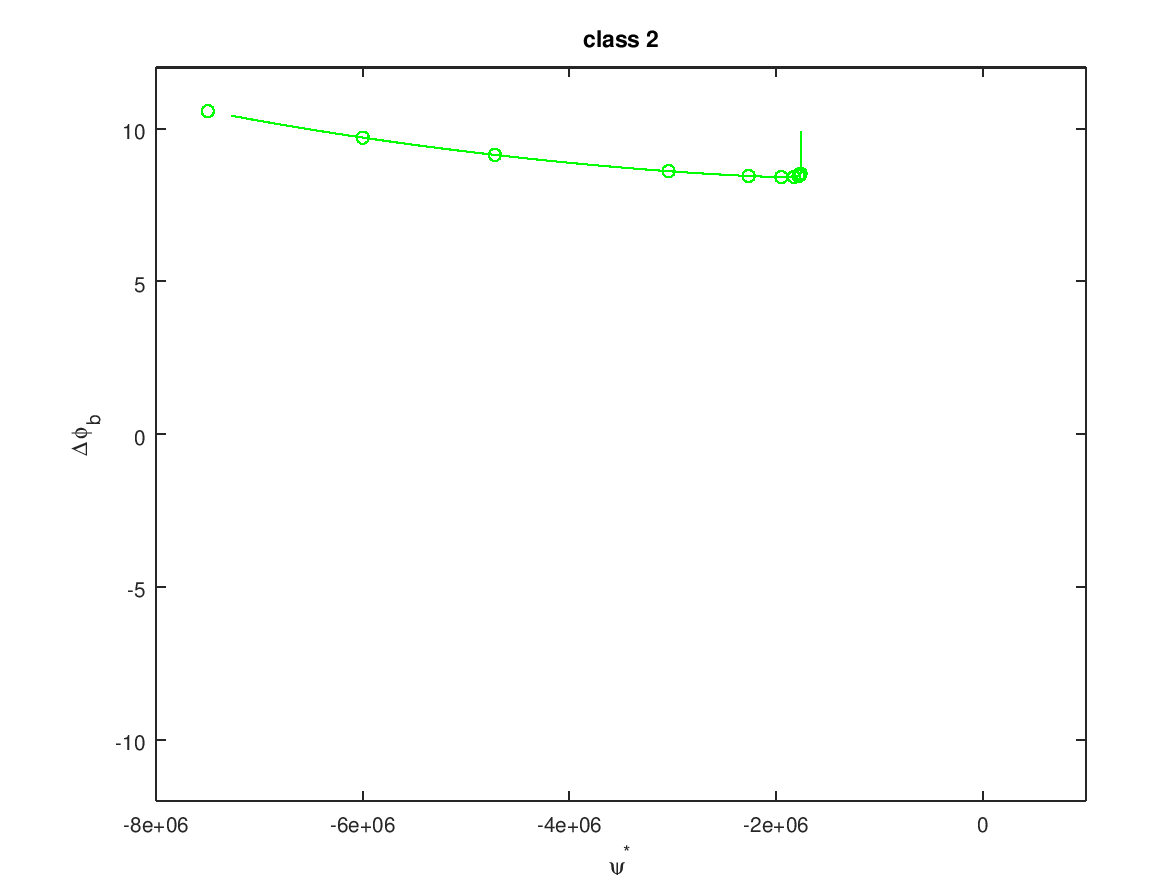
\includegraphics[width=0.33\linewidth]{FIGURES/delphi2}
\includegraphics[width=0.33\linewidth]{FIGURES/delphi3}
}
\centerline{
\includegraphics[width=0.33\linewidth]{FIGURES/delphi4}
\includegraphics[width=0.33\linewidth]{FIGURES/delphi5}
\includegraphics[width=0.33\linewidth]{FIGURES/delphi6}
}
\centerline{
\includegraphics[width=0.33\linewidth]{FIGURES/delphi7}
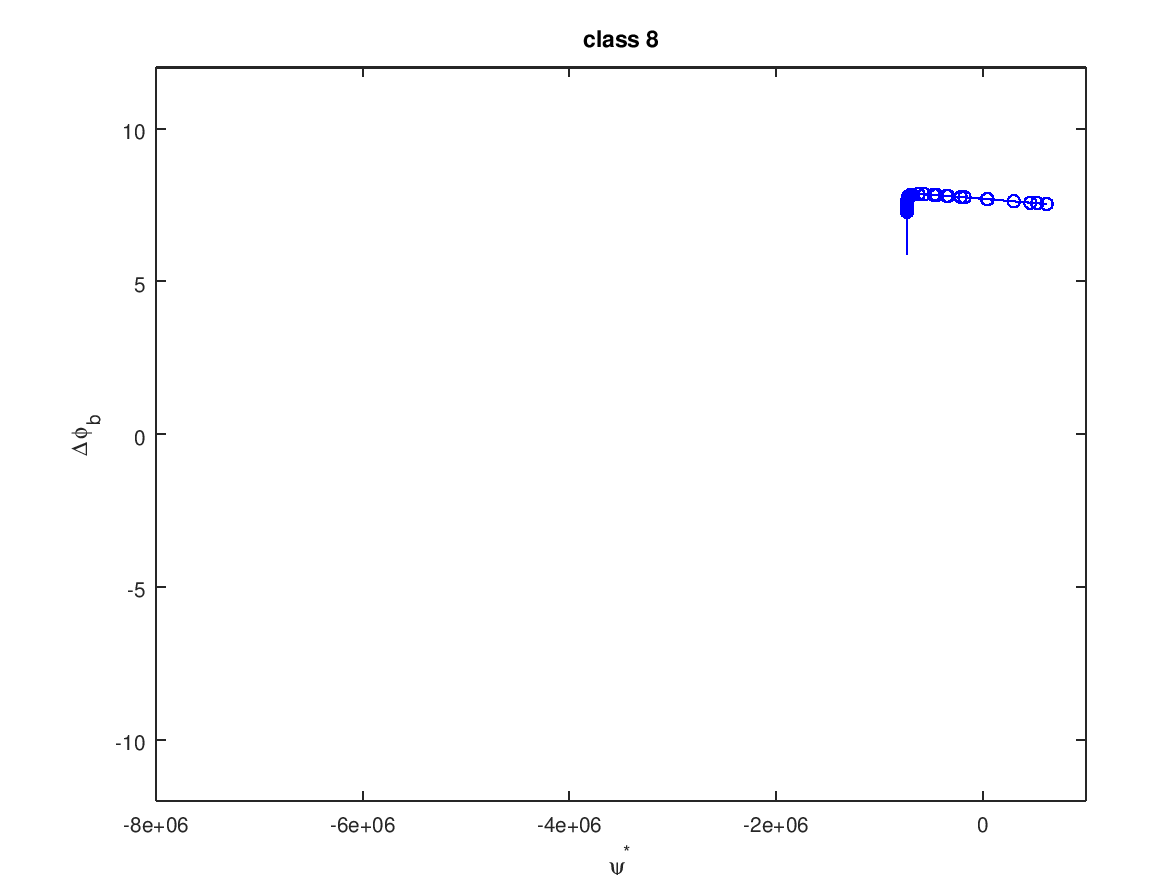
\includegraphics[width=0.33\linewidth]{FIGURES/delphi8}
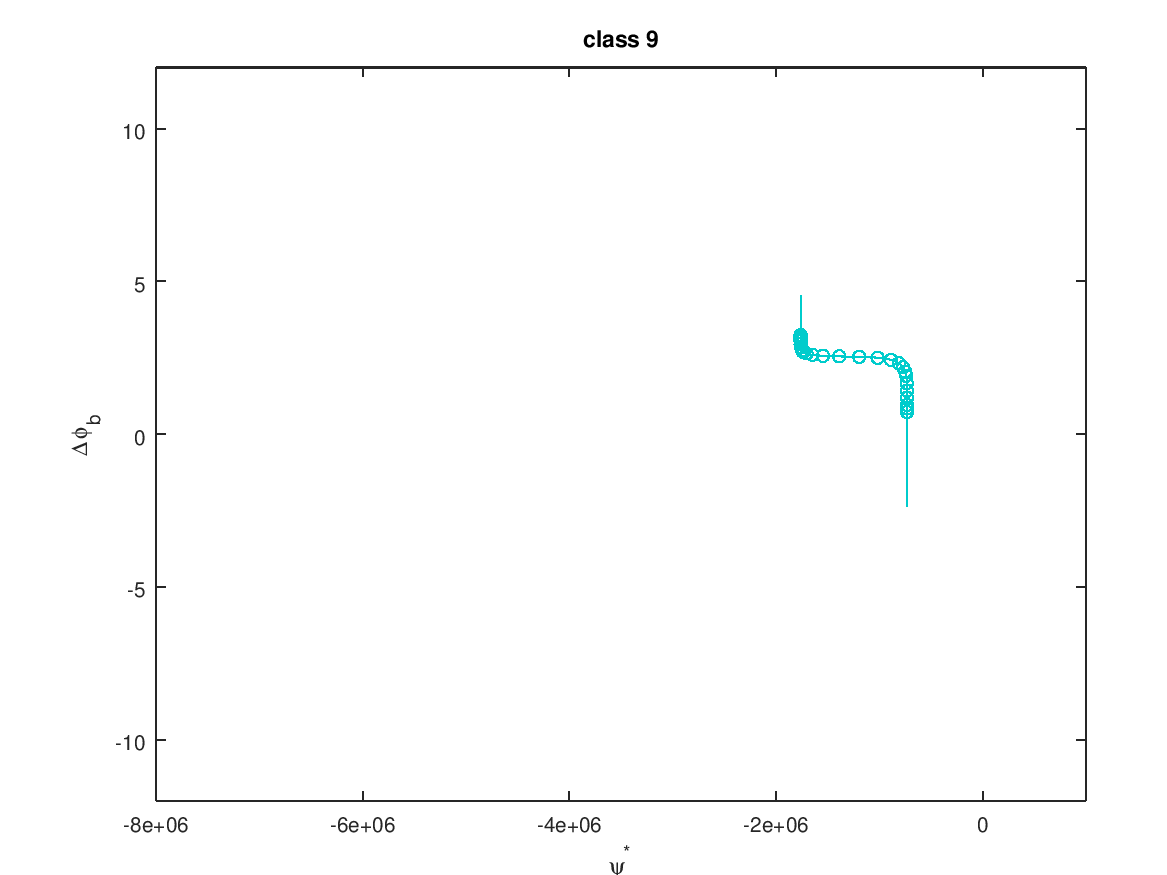
\includegraphics[width=0.33\linewidth]{FIGURES/delphi9}
}
\centerline{
\includegraphics[width=0.33\linewidth]{FIGURES/delphi10}
\includegraphics[width=0.33\linewidth]{FIGURES/delphi_all}
}
\caption[]{
Toroidal displacement $\Delta\varphi_b$ as function of $\psi^\ast$. 
Notation is the same as in Fig.~\ref{fig:taub}.
}
\label{fig:delphi}
\end{figure}

\begin{figure}[ht]
\centerline{
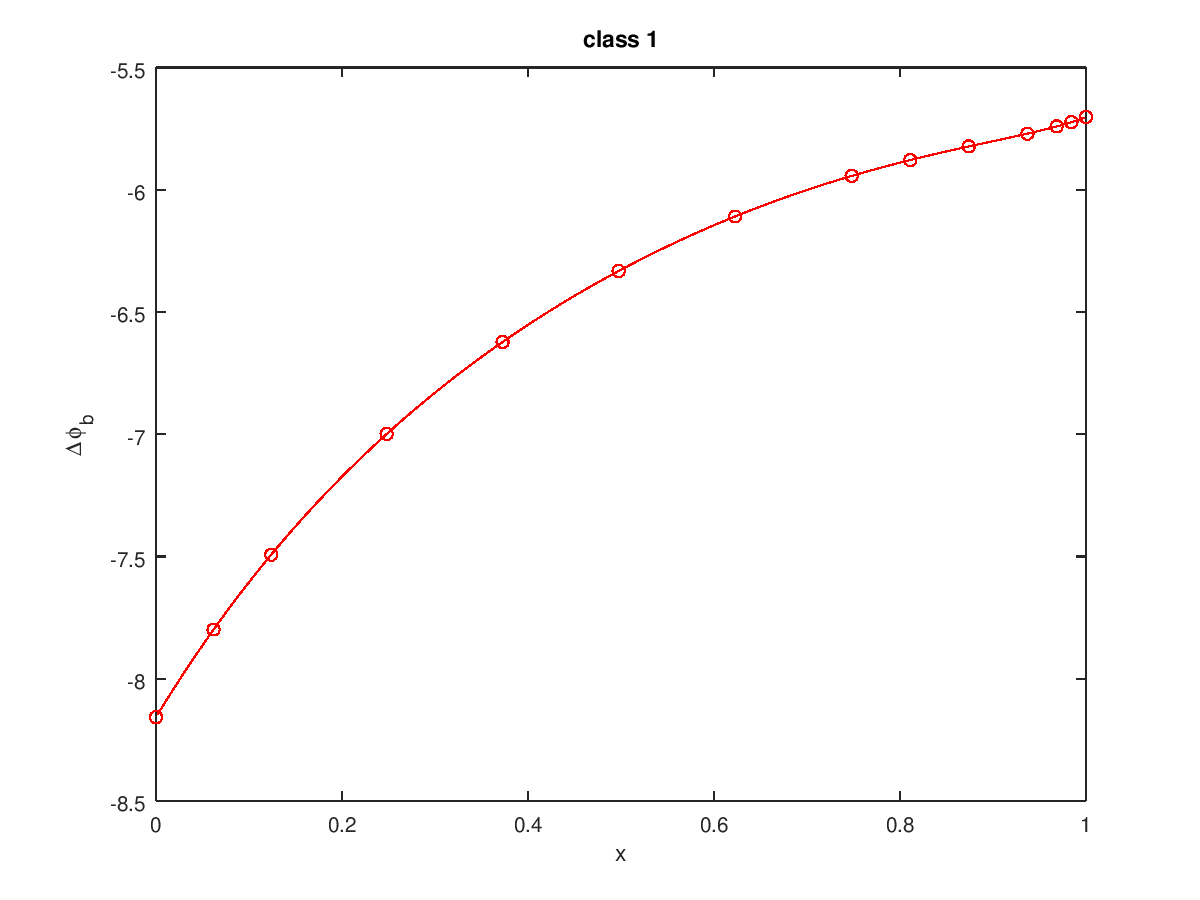
\includegraphics[width=0.33\linewidth]{FIGURES/delphi_x1}
\includegraphics[width=0.33\linewidth]{FIGURES/delphi_x2}
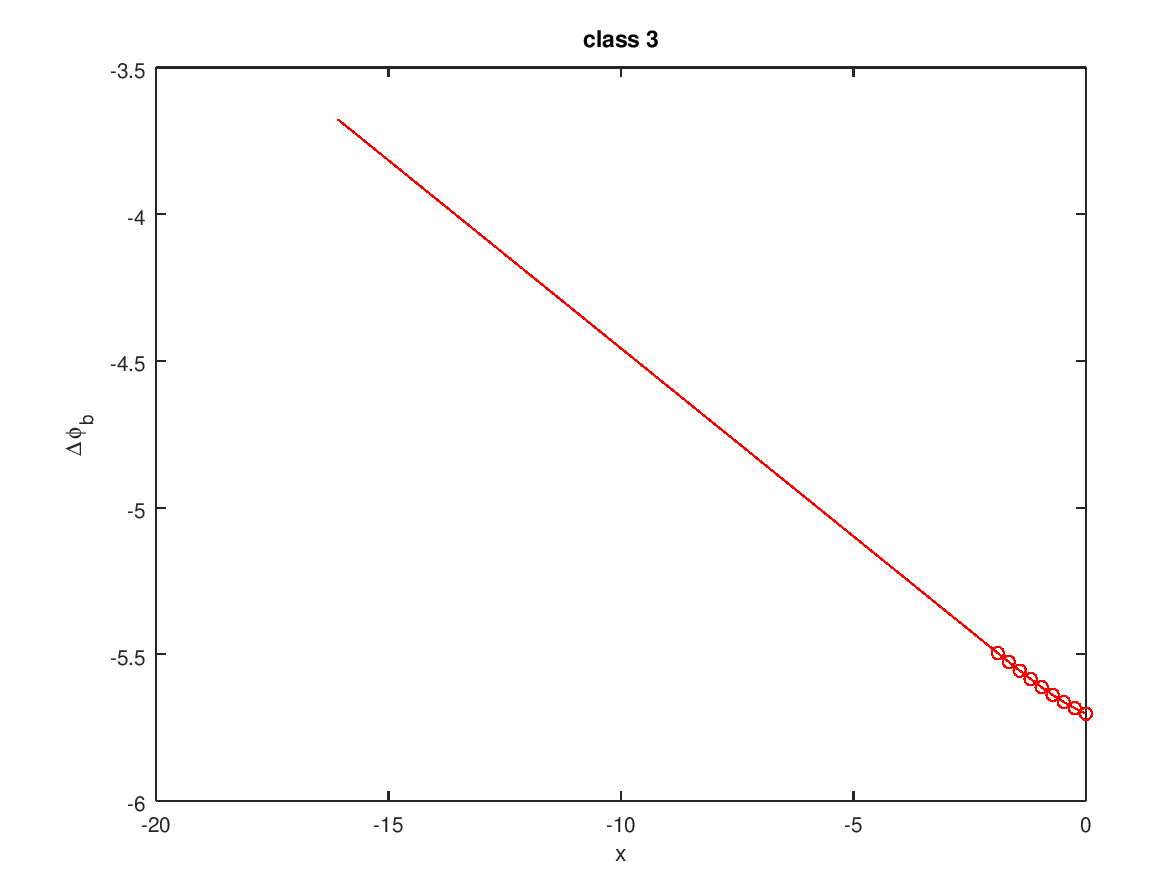
\includegraphics[width=0.33\linewidth]{FIGURES/delphi_x3}
}
\centerline{
\includegraphics[width=0.33\linewidth]{FIGURES/delphi_x4}
\includegraphics[width=0.33\linewidth]{FIGURES/delphi_x5}
\includegraphics[width=0.33\linewidth]{FIGURES/delphi_x6}
}
\centerline{
\includegraphics[width=0.33\linewidth]{FIGURES/delphi_x7}
\includegraphics[width=0.33\linewidth]{FIGURES/delphi_x8}
\includegraphics[width=0.33\linewidth]{FIGURES/delphi_x9}
}
\centerline{
\includegraphics[width=0.33\linewidth]{FIGURES/delphi_x10}
}
\caption[]{
Toroidal displacement $\Delta\varphi_b$ as function of $x$.
Notation is the same as in Fig.~\ref{fig:taub_x}.
}
\label{fig:delphi_x}
\end{figure}

The number of adaptive grid points required to resolve classes 
is given in Table~\ref{tab:gridpoints} for two cases. First case
corresponds to sampling of $\psi^\ast$, $\hat\tau_b$ and 
$\Delta\varphi_b$ only. Second case includes the sampling of 
bounce time integrals of Eq.~\eq{bi_classes_norm} 
%and~\eq{bi_classes_norm_tconst} 
using 6 base functions $\phi_i$.
Base functions in our case are powers of normalized poloidal flux,
\be{testfdef}
\phi_i(r)=r^{i-1},
\qquad
r=\frac{\psi-\psi_{axis}}{\psi_{sep}-\psi_{axis}}=\rho_{\rm pol}^2,
\ee
where $\psi_{axis}$ and $\psi_{sep}$ are poloidal flux values
at the magnetic axis and at the separatrix, respectively.
The number of grid nodes is larger in the second case because
of resolving in addition to the quantities of the first case 
also the dependence of bounce integrals on $\psi^\ast$ which
is relatively steep near $\rho_{\rm pol}$ domain boundary
due to function $\Theta_w$, Eq.~\eq{Theta_W_def}.
\begin{table}[ht]
\centering
\caption{Number of grid points per class.}
\begin{tabular}{| c || c | c | c | c | c | c | c | c | c | c | c |}
\hline
\hline
class index & 1 & 2 & 3 & 4 & 5 & 6 & 7 & 8 & 9 & 10 & total \\
\hline
\hline
number of grid points (frequencies only) &\; 14\; &\; 11\; &\; 9\; &\; 9\; &\; 26\; &\; 26\; &\; 17\; &\; 28\; &\; 26\; &\; 15\; &\; 181\; \\
\hline
number of grid points (equilibrium integrals) &\; 34\; &\; 48\; &\; 9\; &\; 9\; &\; 35\; &\; 29\; &\; 44\; &\; 31\; &\; 28\; &\; 51\; &\; 318\; \\
\hline
\end{tabular}
\label{tab:gridpoints}
\end{table}
It should be noted that case of 10 classes shown here is the most extreme one
for our test configuration with positive radial electric field (see 
section~\ref{ssec:testprof} for more details). Mostly, there are two or five 
classes which, respectively, need less grid points per $\hat J_\perp$ value.

\subsection{Toroidal guiding center rotation velocity}
\label{ssec:torvel}

We should note that toroidal flow of guiding centers~\eq{Vgphi} differs
from actual toroidal flow~\eq{nomegator} by the toroidal component
of Larmor gyration flow, 
\be{larmorflow}
n_\alpha \bV_L = -\nabla\times\frac{p_\perp \bh}{m_\alpha\omega_c},
\ee
where $p_\perp$ is perpendicular pressure and $\bh=\bB/B$.
This flow is divergence free and, therefore, does not contribute to the flux
surface average toroidal flux density however it makes a difference for the
flux surface averaged toroidal flux density which, according to~\eq{tordr}
and~\eq{nomegator} is
\be{torflow}
\left\langle n_\alpha V_\alpha^\varphi(\br) \right\rangle
=\Omega_{\rm tor}(\psi) \left\langle n_\alpha(\psi,\vartheta) \right\rangle
\approx\Omega_{\rm tor}(\psi) \bar n_\alpha(\psi)
=
c 
\left(\bar n_\alpha\difp{\Phi(\psi)}{\psi}
+\frac{T_\alpha}{e_\alpha}\difp{\bar n_\alpha}{\psi}\right).
\ee
Approximate equality stands here for ignoring the centrifugal effect.
Contribution of Larmor flow in this flux density 
is expressed in flux coordinates $(\psi,\vartheta,\varphi)$ 
for the case of constant temperature in $p_\perp=\bar n_\alpha T_\alpha$ 
as follows,
\be{torflow_L}
\left\langle n_\alpha V_{L\alpha}^\varphi(\br) \right\rangle
=
-\frac{cT_\alpha}{e_\alpha}
\left\langle
\frac{1}{\sqrt{g}}\left(
\difp{}{\psi}\frac{\bar n_\alpha B_\vartheta}{B^2}
-
\difp{}{\vartheta}\frac{\bar n_\alpha B_\psi}{B^2}
\right)
\right\rangle
=
-\frac{cT_\alpha}{e_\alpha}
\left(\int\limits_{0}^{2\pi}\rd \vartheta \sqrt{g}\right)^{-1}
\difp{}{\psi} 
\int\limits_{0}^{2\pi}\rd \vartheta \frac{\bar n_\alpha B_\vartheta}{B^2}.
\ee
In Boozer coordinates with $\sqrt{g}=(qB_\varphi+B_\vartheta)/B^2$ Eq.~\eq{torflow_L}
is
\be{torflow_L_booz}
\left\langle n_\alpha V_{L\alpha}^\varphi(\br) \right\rangle
=
-\frac{cT_\alpha}{e_\alpha(qB_\varphi+B_\vartheta)}
\left(\int\limits_{0}^{2\pi}\frac{\rd \vartheta}{B^2}\right)^{-1}
\difp{}{\psi} \bar n_\alpha B_\vartheta
\int\limits_{0}^{2\pi}\frac{\rd \vartheta}{B^2} 
\approx
-\frac{cT_\alpha}{e_\alpha qB_\varphi}\difp{}{\psi} \bar n_\alpha B_\vartheta,
\ee
where we ignored terms quadratic in toroidicity $\varepsilon_t=r/R$ using, in 
particular, $B_\varphi \approx BR$ and $B_\vartheta \approx BR \varepsilon_t/q$.
Comparing~\eq{torflow_L_booz} with~\eq{torflow} we see that this contribution
scales as $(\varepsilon_t/q)^2 \ll 1$ and becomes important only if density
and electrostatic potential gradients are absent or balance each other to zero.
%
\begin{figure}[ht]
\centerline{
\includegraphics[width=0.5\linewidth]{FIGURES/dens}
\includegraphics[width=0.5\linewidth]{FIGURES/torvel}
}
\caption[]{Density (left) and flux surface averaged toroidal flux
density of the guiding centers (right), without electric field (blue), with 
positive electric field (red) and with negative electric field (magenta).
Reference toroidal flux densities (dashed) correspond to the
full flux~\eq{normtorfl}. Green curves correspond to the difference between
respective flows for positive and zero electric field.
}
\label{fig:equiprofs}
\end{figure}
%
In the normalized variables velocities in the code are divided by normalization
velocity $v_0$.
Therefore third of weights $a_0$ in~\eq{a0} is replaced by a normalized
one, $\hat a_{03} = a_{03}/v_0$, and the normalized flow for $\hat T_\alpha = const$ 
is
\be{normtorfl}
\left\langle n_\alpha \hat V_\alpha^\varphi(\br) \right\rangle
=
\frac{1}{v_0}\left\langle n_\alpha V_\alpha^\varphi(\br) \right\rangle
=
\Phi_{\rm eff}
\left(\bar n_\alpha\difp{\hat \Phi(\psi)}{\psi}
+\hat T_\alpha\difp{\bar n_\alpha}{\psi}\right).
\ee
Here we introduced the notation 
\be{Phieff}
\Phi_{\rm eff}=\frac{c {\cal E}_{\rm ref}}{e_\alpha v_0}
\ee
for the effective potential which has nothing to do with actual
electrostatic potential except for the dimension.

\subsection{Test for equilibrium profiles}
\label{ssec:testprof}

For testing, we use AUG equilibrium g30835.3200\_ed6. We use deuterium ions
with constant temperature $T_d = 5$ keV. Profiles of density parameter
of the Maxwellian and of the normalized electrostatic potential are
\be{equi_input}
\bar n_d(\psi) = 1 - r,
\qquad
\hat \Phi(\psi) = \hat\Phi_A \left(r -\frac{r^2}{2}+\frac{r^3}{4}\right),
\ee
where flux surface label $r=r(\psi)$ is a square of the normalized poloidal 
radius~\eq{testfdef}. We use 3 values of the amplitude $\hat\Phi_A$: zero
for no electric field, -1.12 for positive radial electric field and -1.12 for
negative electric field. All illustrations in 
Figs.~\ref{fig:psiast}-\ref{fig:delphi_x} of the previous sections
correspond to the case of positive electric field.

In Fig.~\ref{fig:equiprofs}, the results of three above cases are shown for
the density and toroidal flow density profiles. In case of finite orbits widths,
actual density $n_d$ needs not to be the same with Maxwellian density parameter
$\bar n_d$. Nevertheless, since $n_d$ and $\bar n_d$ agree very well in absence
of electric field, differences for the finite electric field are due to the
computational error.

As seen from Fig.~\ref{fig:equiprofs}, 
difference between the full toroidal flow~\eq{normtorfl} and flow of the guiding 
centers computed by orbit integration is small as expected due to the smallness of
Larmor flow~\eq{torflow_L_booz}. Larmor flow should vanish completely from the 
results if one takes a difference between two flows computed for the same density
profiles but different electric fields. This is seen from green curves which differ
only by the numerical error.

\subsection{Quasilinear flux}
Quasilinear box-integrated flux density~\eq{boxflux_classes_conv}
takes for the equilibrium Maxwellian distribution
the following form in the normalized variables,
\bea{boxflux_classes_norm}
\Gamma_{\rm box}(r_0) &=&
-\frac{\pi^{3/2}}{4} v_0\sum_\bm |m_3|
\int\limits_{\hat\Phi_{\rm min}}^\infty \rd \hat H_0
\int\limits_0^{\hat J_\perp^{\rm max}(\hat H_0)} \rd \hat J_\perp
\sum\limits_{k=1}^{N_{\rm cl}}
\int\limits_{x^{[min]}_k}^{x^{[max]}_k} \rd x
\left|\difp{\psi^\ast}{x}\right|
\;\left|\hat H_{\bm}\right|^2
\delta\left(\Delta\varphi_b+\frac{2\pi m_2}{m_3}\right)\;
\nonumber \\
&\times&
\left(
\Phi_{\rm eff}
\left(
A^\ast_1(\psi^\ast)+
\frac{\hat H_0-\hat \Phi(\psi^\ast)}{\hat T_\alpha}
A^\ast_2(\psi^\ast) 
\right)
\hat \tau_b
+\frac{1}{\hat T_\alpha}\Delta\varphi_b
\right)
\frac{\bar n_\alpha(\psi^\ast)}{\hat T_\alpha^{3/2}}
\exp\left(\frac{\hat \Phi(\psi^\ast)-\hat H_0}{\hat T_\alpha}\right)
\nonumber \\
&\times&
\left\langle
\left(
\hat\tau_b \Phi_{\rm eff}
\left(\difp{r}{\psi^\ast}\right)_{\theta^2}
-\Delta\varphi_b\left(\difp{r}{\hat H_0}\right)_{\psi^\ast,\theta^2}
\right)\Theta(r_0-r)
\right\rangle_b,
\eea
where Fourier amplitude of the perturbed Hamiltonian is 
normalized similarly to the unperturbed Hamiltonian,
\be{hatHbm}
\hat H_\bm = \frac{H_\bm}{{\cal E}_{\rm ref}},
\ee
normalizing constant $\Phi_{\rm eff}$ and dimensionless temperature $\hat T_\alpha$
are defined by Eq.~\eq{Phieff} and~\eq{That}, respectively, 
and non-local thermodynamic forces are
\be{nl_themforces}
A^\ast_1(\psi^\ast)=\frac{1}{\bar n_\alpha}
\difp{\bar n_\alpha}{\psi^\ast}
+\frac{1}{\hat T_\alpha} \difp{\hat\Phi}{\psi^\ast}
-\frac{3}{2\hat T_\alpha}\difp{\hat T_\alpha}{\psi^\ast},
\qquad
A^\ast_2(\psi^\ast)=\frac{1}{\hat T_\alpha}\difp{\hat T_\alpha}{\psi^\ast}.
\ee
The normalized bounce average in~\eq{boxflux_classes_norm} can similarly
to~\eq{bouav_theta} and~\eq{bouav_theta_cx} be presented in the form
\bea{bouav_theta_norm}
&&
\left\langle
\left(
\hat\tau_b \Phi_{\rm eff}
\left(\difp{r}{\psi^\ast}\right)_{\theta^2}
-\Delta\varphi_b\left(\difp{r}{\hat H_0}\right)_{\psi^\ast,\theta^2}
\right)\Theta(r_0-r)
\right\rangle_b
\nonumber \\
&&\qquad\qquad
=
\frac{1}{2}
\left(
\Phi_{\rm eff}
\left(\hat\tau_b -\frac{h_\varphi}{\hat v_\parallel}\right)
\left(\difp{\psi^\ast}{x}\right)^{-1}\difp{}{x}
-\Delta\varphi_b\left(\difp{}{\hat H_0}\right)_x
\right)
\left\langle
r_0-r+|r_0-r|
\right\rangle_b
\nonumber \\
&&\qquad\qquad
=
\left(
\Phi_{\rm eff}
\left(\hat\tau_b -\frac{h_\varphi}{\hat v_\parallel}\right)
\left(\difp{\psi^\ast}{x}\right)^{-1}\difp{}{x}
-\Delta\varphi_b\left(\difp{}{\hat H_0}\right)_x
\right)
\left\langle
\left(r_0-r\right)\Theta(r_0-r)
\right\rangle_b.
\eea
It may be more practical not to use class parameterisation varible $x$
which, for fixed $R_c$, depends on the integrals of motion. In case one
needs to evaluate~\eq{bouav_theta_norm} in between the pre-computed
grid nodes over $\hat J_\perp$, it is better to use cut parameter $R_c$
directly, so that
\bea{bouav_theta_norm_Rc}
&&
\left\langle
\left(
\hat\tau_b \Phi_{\rm eff}
\left(\difp{r}{\psi^\ast}\right)_{\theta^2}
-\Delta\varphi_b\left(\difp{r}{\hat H_0}\right)_{\psi^\ast,\theta^2}
\right)\Theta(r_0-r)
\right\rangle_b
\nonumber \\
&&\qquad\qquad
=
\left(
\Phi_{\rm eff}
\left(\hat\tau_b -\frac{h_\varphi}{\hat v_\parallel}\right)
\left(\difp{\psi^\ast}{R_c}\right)^{-1}\difp{}{R_c}
-\Delta\varphi_b\left(\difp{}{\hat H_0}\right)_{R_c}
\right)
\left\langle
\left(r_0-r\right)\Theta(r_0-r)
\right\rangle_b,
\eea
and
$$
\difp{\psi^\ast}{R_c}=\difp{\psi^\ast}{x}\left(\difp{R_c}{x}\right)^{-1}
$$
is used in the form of interpolation over $\hat J_\perp$.

According to Eq.(27) of C.G.Albert et al, PoP {\bf 23}, 082515 (2016),
the normalized perturbed Hamiltonian is expressed via perturbation
of magnetic field strength $\delta B$ as follows,
\be{normperham}
\delta\hat H = \frac{\delta H}{\cE_{\rm ref}}
=\left(2\left(\hat H_0-\hat\Phi\right)-\hat J_\perp B
\right)\frac{\delta B}{B},
\ee
where $B$ denotes the axisymmetric part of the perturbed field which is
approximately the same with the unperturbed field and which is used for the
computation of ``unperturbed'' orbits.
Presenting perturbation of magnetic field as a Fourier series
\be{bmodfour}
\delta B = {\rm Re}\sum\limits_{n=1}^\infty B_n(R,Z){\rm e}^{in\varphi},
\ee
we get for the Fourier amplitude~\eq{hatHbm} for $\bm=(0,m_2,m_3)$
\bea{hatBm_get}
\hat H_\bm 
&=& \left\langle 
\left(2\left(\hat H_0-\hat\Phi\right)-\hat J_\perp B
\right)\frac{B_{m_3}}{B}{\rm e}^{im_3\varphi-i(m_2\omega_b+m_3\Omega_\varphi)\tau}
\right\rangle_b
\nonumber \\
&=& \left\langle 
\left(2\left(\hat H_0-\hat\Phi\right)-\hat J_\perp B
\right)\frac{B_{m_3}}{B}{\rm e}^{im_3\varphi}
\right\rangle_b,
\eea
where $\hat\Phi=\hat\Phi(\cR,\cZ)$, $B=B(\cR,\cZ)$ and $B_{m_3}=B_{m_3}(\cR,\cZ)$
are functions of the orbit,
and we used the resonance condition $m_2\omega_b+m_3\Omega_\varphi=0$ in the
last expression. For the numerical evaluation of~\eq{hatBm_get} it is important
that last bounce averaged expression is a periodic function of orbit parameter 
$\hat\tau$ with period $\hat\tau_b$. This is not exactly the case when the resonance
condition is solved numerically using interpolation of $\Delta\varphi_b$. Therefore,
evaluation of~\eq{hatBm_get} is done in two steps: first, bunce time $\hat\tau_b$
and toroidal displacement $\Delta\varphi_b$ are computed for approximate starting
conditions $(\hat H_0,\hat J_\perp, x)$ of the resonant orbit, and then bounce 
average~\eq{hatBm_get} is computed for these condition using the newly computed
$\hat\tau_b$ and $\Delta\varphi_b$ in the first expression~\eq{hatBm_get} 
which is periodic for any orbit, not necessarily the resonant one. 
Thus, normalized Fourier amplitude of the perturbed Hamiltonian in normalized 
variables is
\be{hatBm_norm}
\hat H_\bm
= \left\langle
\left(2\left(\hat H_0-\hat\Phi\right)-\hat J_\perp B
\right)\frac{B_{m_3}}{B}
\exp\left
(im_3\varphi-i(2\pi m_2+m_3\Delta\varphi_b)\frac{\hat\tau}{\hat\tau_b}
\right)
\right\rangle_b.
\ee

Finally, there are few methods to integrate over phase space
in Eq.~\eq{boxflux_classes_norm}:
\begin{itemize}
\item[1]
The most straightforward one is to evaluate integral over 
$x$ in~\eq{boxflux_classes_norm} using the $\delta$-function which gives
\bea{boxflux_classes_norm_evald}
\Gamma_{\rm box}(r_0) &=&
-\frac{\pi^{3/2}}{4} v_0
\int\limits_{\hat\Phi_{\rm min}}^\infty \rd \hat H_0
\int\limits_0^{\hat J_\perp^{\rm max}(\hat H_0)} \rd \hat J_\perp
\sum\limits_{k=1}^{N_{\rm cl}}
\sum_\bm |m_3|
\sum_{x=x^{(\rm res)}_{(\bm,k)}}
\left|\difp{\psi^\ast}{x}\right|
\left|\difp{\Delta \varphi_b}{x}\right|^{-1}
\;\left|\hat H_{\bm}\right|^2
\nonumber \\
&\times&
\left(
\Phi_{\rm eff}
\left(
A^\ast_1(\psi^\ast)+
\frac{\hat H_0-\hat \Phi(\psi^\ast)}{\hat T_\alpha}
A^\ast_2(\psi^\ast)
\right)
\hat \tau_b
+\frac{1}{\hat T_\alpha}\Delta\varphi_b
\right)
\frac{\bar n_\alpha(\psi^\ast)}{\hat T_\alpha^{3/2}}
\exp\left(\frac{\hat \Phi(\psi^\ast)-\hat H_0}{\hat T_\alpha}\right)
\nonumber \\
&\times&
\left\langle
\left(
\hat\tau_b \Phi_{\rm eff}
\left(\difp{r}{\psi^\ast}\right)_{\theta^2}
-\Delta\varphi_b\left(\difp{r}{\hat H_0}\right)_{\psi^\ast,\theta^2}
\right)\Theta(r_0-r)
\right\rangle_b,
\eea
where we denote with summation over $x=x^{(\rm res)}_{(\bm,k)}$ sum over
all resonant values of $x$ for a given class $k$ and fixed Fourier indices $\bm$,
and all finctions of $\psi^\ast=\psi^\ast(x)$ resonant values of $x$ are used.
This method may result in steep behaviour and integrable square root singularities 
of the subintegrand over $\hat J_\perp$ because of U-turns of the resonant line
in $(\hat J_\perp,x)$ plane. This may require special integration procedure.
\item[2]
Use some more clever method of integration along the line in $(\hat J_\perp,x)$ plane.
This can be done in separate $\hat J_\perp$ intervals where a set of classes does not 
change, i.e. no new class appears and no existing class disappears when changing
$\hat J_\perp$. 
In these regions, one can generate the data on a fine equidistant grid 
in $x$ using the adaptive interpolation, and use usual 2D interpolation over
$(\hat J_\perp,x)$ since the boundaries of $x$ interval do not depend on 
$\hat J_\perp$. Such an approach will need some logics in order to find proper
$\hat J_\perp$ intervals of those regions.

\end{itemize}
%
\begin{figure}[ht]
\centerline{
\includegraphics[width=0.4\linewidth]{FIGURES/res_total}
\includegraphics[width=0.4\linewidth]{FIGURES/res_total_zoom}
}
\caption[]{
Subintegrand in Eq.~\eq{boxflux_classes_norm_evald} as function of normalized
perpendicular invariant $\hat J_\perp$ and fixed $\hat H_0=1$ 
for zero (blue), positive (red) and 
negative(green) radial electric field. Right picture is zoom of the region where
subintegrands differ from zero.
}
\label{fig:restot}
\end{figure}

\subsubsection{Method 1}
\label{sssec:one}
%
%
\begin{figure}[ht]
\centerline{
\includegraphics[width=0.4\linewidth]{FIGURES/res_noE_modes}
\includegraphics[width=0.4\linewidth]{FIGURES/res_noE_modes_zoom}
}
\centerline{
\includegraphics[width=0.4\linewidth]{FIGURES/res_E_modes}
\includegraphics[width=0.4\linewidth]{FIGURES/res_E_modes_zoom}
}
\centerline{
\includegraphics[width=0.4\linewidth]{FIGURES/res_mE_modes}
\includegraphics[width=0.4\linewidth]{FIGURES/res_mE_modes_zoom}
}
\caption[]{
Total subintegrand in Eq.~\eq{boxflux_classes_norm_evald} 
(same as in Fig.~\ref{fig:restot} here with dotted black) and contributions
from various bounce modes $m_2$ indicated in the legend.
Cases with zero, positive and negative radial electric field are shown in upper,
middle and lower panels, respectively. Right pictures are zoom of the 
regions with singular behaviour.
}
\label{fig:restot_modes}
\end{figure}
%
%
In Figs.~\ref{fig:restot} and~\ref{fig:restot_modes} the results are shown for the
subintegrand in Eq.~\eq{boxflux_classes_norm_evald} (excluding factor $v_0$ in front)
for the same profiles of equilibrium density and electrostatic potential as before.
This subintegrand is plotted for the fixed normalized total energy 
$\hat H_0 = 0.996 \approx 1$ as a function of normalized perpendicular invariant
$\hat J_\perp$ using 5000 equidistant grid points. This is the amount comparable
to the number of points in 2D grid for the equilibrium profile test (60x50).

As expected, behaviour of the subintegrand is complicated: it has discontinuities 
and singularities. In case of U-turns of the resonant line, 
$y-x^2=0$ with integration over $x$, these singularities are integrable as $y^{-1/2}$.
Generally, they stay integrable also for general curvatures of a kind $y-x^m=0$
since the result of integration over $x$ scales as $y^{1-1/m}$. In particular, 
this is true for the inflection points, $m=3$.

Multiple sigularities in total subintegrand shown in Fig.~\ref{fig:restot}
come from separate bounce harmonics as it can be seen in Fig.~\ref{fig:restot_modes}.
All these harmonics are computed simultaneously using the same adaptive interpolation
of frequencies which is the main CPU time consumer.

Generally, we may conclude that method 1 is feasible but requires a custom adaptive
integrator which can handle integrable singularities. Usual equidistant integration
requires a large number of points (5000 in this example would result in days of run
for the whole integral). Adaptive integrator should reduce this number by more than 
an order of magnitude.

\end{document}
